\documentclass{cas-sc}

\usepackage{caption}
\usepackage{subcaption}

\usepackage{siunitx}
\sisetup{per-mode=symbol,range-units=single,range-phrase=--}

\usepackage{pgfplots}
\pgfplotsset{compat=newest}
\definecolor{colorblind0}{RGB}{1,115,178}
\definecolor{colorblind1}{RGB}{222,143,5}
\definecolor{colorblind2}{RGB}{2,158,115}
\newcommand{\epyfigurewidth}{\linewidth}
\newcommand{\epyheightratio}{0.85}

\begin{document}

\title[mode=title]{VQhull: A Fast Planar Quickhull}
\shorttitle{VQhull: A Fast Planar Quickhull}
\shortauthors{T. Koopman et~al.}

\appendix

\begin{table}
  \centering
  \begin{tabular}{lrrrrrrrrr}
    & \multicolumn{3}{c}{cn125} & \multicolumn{3}{c}{cn132} & \multicolumn{3}{c}{laptop} \\
    & Circle & Disk & Kuzmin & Circle & Disk & Kuzmin & Circle & Disk & Kuzmin \\\midrule
    PBBS seq & 60.75 & 3.85 & 0.99 & 39.02 & 2.96 & 0.57 & 29.64 & 2.13 & 0.58 \\
    VQhull seq & 3.85 & 0.45 & 0.32 & 7.24 & 0.81 & 0.58 & 4.38 & 0.50 & 0.31 \\
    PBBS par & 10.70 & 0.63 & 0.22 & 3.31 & 0.19 & 0.07 & 8.46 & 0.59 & 0.17 \\
    VQhull par & 1.42 & 0.24 & 0.14 & 0.33 & 0.07 & 0.05 & 1.61 & 0.17 & 0.11 \\
  \end{tabular}
  \caption{VQhull and PBBS mean runtime in seconds per system and per dataset.
  For the sequential implementations and the parallel implementations using all
  available threads.}
\end{table}

\begin{table}
  \centering
  \begin{tabular}{lrrrrrrrrr}
    & \multicolumn{3}{c}{cn125} & \multicolumn{3}{c}{cn132} & \multicolumn{3}{c}{laptop} \\
    & Circle & Disk & Kuzmin & Circle & Disk & Kuzmin & Circle & Disk & Kuzmin \\\midrule
    PBBS seq & 1.2 & 1.9 & 5.7 & 1.9 & 2.4 & 9.9 & 2.5 & 3.4 & 9.7 \\
    VQhull seq & 18.9 & 16.1 & 17.7 & 10.1 & 8.9 & 9.7 & 16.7 & 14.6 & 18.1 \\
    PBBS par & 6.8 & 11.4 & 25.2 & 22.0 & 37.6 & 77.5 & 8.6 & 12.3 & 33.0 \\
    VQhull par & 51.5 & 30.2 & 38.7 & 220.7 & 105.4 & 117.7 & 45.4 & 42.2 & 51.9 \\
  \end{tabular}
  \caption{VQhull and PBBS mean bandwidth in \si{\giga\byte\per\second} per
  system and per dataset. For the sequential implementations and the parallel
  implementations using all available threads.}
\end{table}

\begin{table}
  \centering
  \begin{tabular}{lrrrrrrrrr}
    & \multicolumn{3}{c}{cn125} & \multicolumn{3}{c}{cn132} & \multicolumn{3}{c}{laptop} \\
    & Circle & Disk & Kuzmin & Circle & Disk & Kuzmin & Circle & Disk & Kuzmin \\\midrule
    PBBS seq & 2.9 & 4.6 & 13.8 & 1.3 & 1.7 & 7.1 & 4.7 & 6.5 & 18.6 \\
    VQhull seq & 46.2 & 39.2 & 43.3 & 7.2 & 6.4 & 7.0 & 32.1 & 28.0 & 34.8 \\
    PBBS par & 16.6 & 27.7 & 61.6 & 15.7 & 26.9 & 55.4 & 16.6 & 23.6 & 63.4 \\
    VQhull par & 125.5 & 73.6 & 94.5 & 157.6 & 75.3 & 84.1 & 87.3 & 81.1 & 99.8 \\
  \end{tabular}
  \caption{VQhull and PBBS mean bandwidth utilization \si{\percent} per system
  and per dataset. For the sequential implementations and the parallel
  implementations using all available threads.}
\end{table}

\begin{table}
  \centering
  \begin{tabular}{lrrrrrrrrr}
    & \multicolumn{3}{c}{cn125} & \multicolumn{3}{c}{cn132} & \multicolumn{3}{c}{laptop} \\
    & Circle & Disk & Kuzmin & Circle & Disk & Kuzmin & Circle & Disk & Kuzmin \\\midrule
    PBBS seq & 820.5 & 52.5 & 13.4 & 831.0 & 61.9 & 13.5 & 805.0 & 58.5 & 15.4 \\
    VQhull seq & 57.6 & 7.0 & 4.8 & 146.7 & 18.0 & 13.1 & 128.9 & 15.0 & 9.2 \\
    PBBS par & 381.1 & 22.9 & 8.5 & 506.9 & 31.0 & 12.7 & 330.3 & 23.5 & 10.3 \\
    VQhull par & 41.3 & 8.3 & 6.0 & 64.2 & 11.4 & 7.6 & 69.0 & 10.7 & 7.2 \\
  \end{tabular}
  \caption{VQhull and PBBS median energy consumption in joules per system and
  per dataset. For the sequential implementations and the parallel
  implementations using all available threads.}
\end{table}

\begin{table}
  \centering
  \begin{tabular}{lrrrrrr}
    & \multicolumn{6}{c}{laptop} \\
    & Circle & IQR & Disk & IQR & Kuzmin & IQR \\\midrule
    PBBS seq & 677.21 & 3006.58 & 3.33 & 11.06 & 1.17 & 2.82 \\
    VQhull seq & 26.85 & 306.91 & 0.45 & 9.47 & 2.79 & 4.38 \\
    PBBS par & 0.00 & 6.76 & 0.28 & 2.27 & 0.00 & 1.06 \\
    VQhull par & 0.00 & 0.00 & 0.00 & 1.14 & 0.10 & 0.43 \\
  \end{tabular}
  \caption{VQhull and PBBS median uncore energy consumption in milli-joules for
  laptop per dataset. For the sequential implementations and the parallel
  implementations using all available threads.}
\end{table}

\begin{figure}
  \scriptsize
  \begin{subfigure}{.333\linewidth}
    \centering
    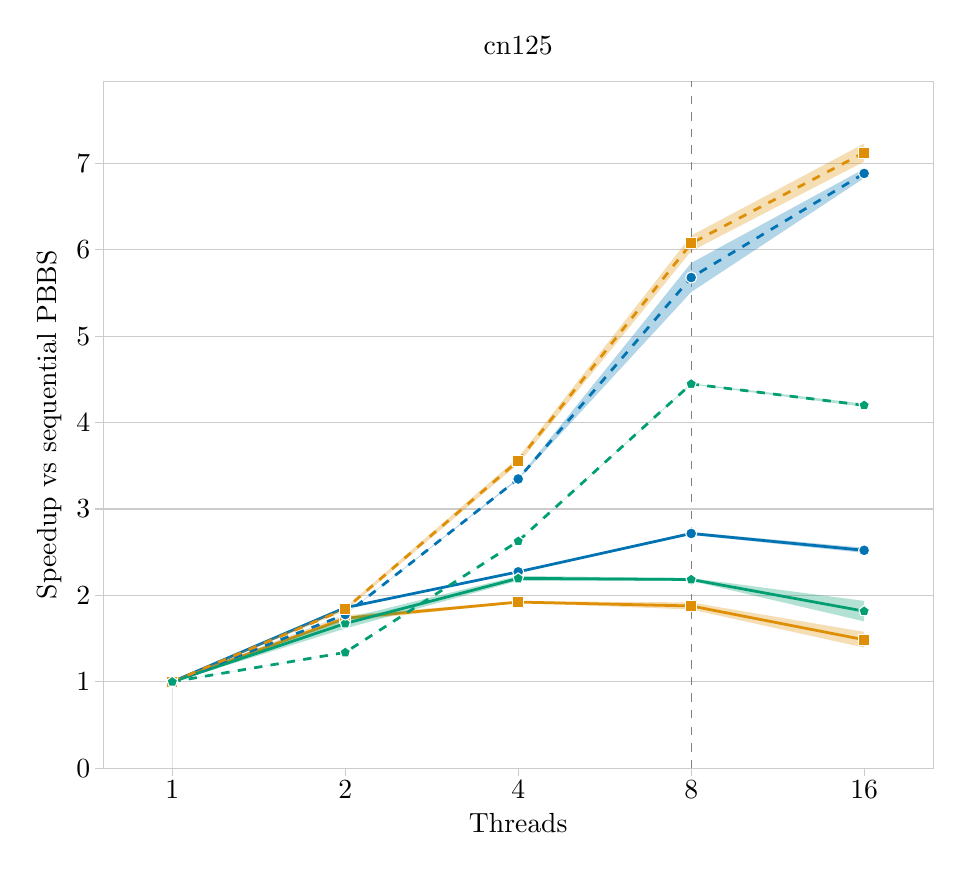
\begin{tikzpicture}
\begin{axis}[
  title={cn125},
  width=\epyfigurewidth,
  height={\epyheightratio*\epyfigurewidth},
  ymin=0,
  xlabel={Threads},
  ylabel={Speedup vs sequential PBBS},
  xmode=log,
  scaled ticks=false,
  xtick={1,2,4,8,16},
  extra y ticks={\pgfkeysvalueof{/pgfplots/ymax}},
  xticklabels={1,2,4,8,16},
  extra y tick labels={\vphantom{Ag}},
  tick pos=left,
  tick align=outside,
  ymajorgrids,
  legend cell align=left,
  major tick length=0.3em,
  /pgf/number format/fixed,
  axis line style={color=black!20},
  y grid style={color=black!20,line width=0.4pt},
  tick style={color=black!20,line width=0.4pt},
  tick label style={inner sep=0.15em},
  ylabel style={outer sep=-0.25em},
  extra y tick style={grid=none,major tick length=0pt,yticklabel style={opacity=0,text opacity=0}},
  legend style={draw=black!20,draw opacity=1,fill opacity=0.9,text opacity=1,inner sep=0.2em},
  legend image code/.code={\path[#1] (0em,0pt) -- (1.4em,0pt) plot coordinates {(0.7em,0pt)};},
]
\addplot[draw=none,fill=colorblind0,fill opacity=0.3,forget plot] coordinates {
  (1,1.0029134559156205)
  (2,1.868443846206898)
  (4,2.27924779405967)
  (8,2.733129344124862)
  (16,2.552036673922606)
  (16,2.4922087715810797)
  (8,2.7009149173753872)
  (4,2.266642999466215)
  (2,1.8481919720928675)
  (1,0.9971025920885291)
} \closedcycle;
\addplot[color=colorblind0,line width=1pt,mark=*,mark size=2pt,mark options={draw=white,line width=-0.4pt,solid}] coordinates {
  (1,1.0000080240020748)
  (2,1.8583179091498827)
  (4,2.2729453967629425)
  (8,2.7170221307501246)
  (16,2.522122722751843)
};
\addplot[draw=none,fill=colorblind1,fill opacity=0.3,forget plot] coordinates {
  (1,1.004128603081254)
  (2,1.7701975465805)
  (4,1.9328453034226312)
  (8,1.9188462688317796)
  (16,1.5778931766344464)
  (16,1.395777364795442)
  (8,1.8368615500854937)
  (4,1.9130658041467592)
  (2,1.7010789823953338)
  (1,0.9959036030749914)
} \closedcycle;
\addplot[color=colorblind1,line width=1pt,mark=square*,mark size=2pt,mark options={draw=white,line width=-0.4pt,solid}] coordinates {
  (1,1.0000161030781227)
  (2,1.735638264487917)
  (4,1.9229555537846952)
  (8,1.8778539094586366)
  (16,1.4868352707149441)
};
\addplot[draw=none,fill=colorblind2,fill opacity=0.3,forget plot] coordinates {
  (1,1.0070217954069982)
  (2,1.732442476438661)
  (4,2.225758756130108)
  (8,2.2006010270069067)
  (16,1.9361483667095278)
  (16,1.6992792824214167)
  (8,2.1678313723044607)
  (4,2.1694074033342328)
  (2,1.6167313270913695)
  (1,0.9930707861070529)
} \closedcycle;
\addplot[color=colorblind2,line width=1pt,mark=pentagon*,mark size=2pt,mark options={draw=white,line width=-0.4pt,solid}] coordinates {
  (1,1.0000462907570256)
  (2,1.6745869017650152)
  (4,2.1975830797321705)
  (8,2.1842161996556837)
  (16,1.8177138245654723)
};
\addplot[draw=none,fill=colorblind0,fill opacity=0.3,forget plot] coordinates {
  (1,1.0017298109663586)
  (2,1.7807859905464074)
  (4,3.357661311580416)
  (8,5.848968691544964)
  (16,6.938667884795825)
  (16,6.832216388760044)
  (8,5.512236605544653)
  (4,3.3385665493759324)
  (2,1.776104831686446)
  (1,0.9982758716319274)
} \closedcycle;
\addplot[color=colorblind0,line width=1pt,dashed,mark=*,mark size=2pt,mark options={draw=white,line width=-0.4pt,solid}] coordinates {
  (1,1.000002841299143)
  (2,1.7784454111164267)
  (4,3.348113930478174)
  (8,5.6806026485448085)
  (16,6.885442136777934)
};
\addplot[draw=none,fill=colorblind1,fill opacity=0.3,forget plot] coordinates {
  (1,1.0010732305591452)
  (2,1.862676929837921)
  (4,3.594669028811271)
  (8,6.165995573186675)
  (16,7.23155171555311)
  (16,7.022185533557968)
  (8,5.985658156403718)
  (4,3.5213619442316992)
  (2,1.8208424264926062)
  (1,0.9989289541851012)
} \closedcycle;
\addplot[color=colorblind1,line width=1pt,dashed,mark=square*,mark size=2pt,mark options={draw=white,line width=-0.4pt,solid}] coordinates {
  (1,1.0000010923721232)
  (2,1.8417596781652636)
  (4,3.558015486521485)
  (8,6.0758268647951965)
  (16,7.126868624555539)
};
\addplot[draw=none,fill=colorblind2,fill opacity=0.3,forget plot] coordinates {
  (1,1.0015509731450785)
  (2,1.3404385845979805)
  (4,2.6288680976036827)
  (8,4.45495185012072)
  (16,4.219230949330616)
  (16,4.183642031695933)
  (8,4.441977883602901)
  (4,2.626890140986997)
  (2,1.339692824761511)
  (1,0.9984535907570137)
} \closedcycle;
\addplot[color=colorblind2,line width=1pt,dashed,mark=pentagon*,mark size=2pt,mark options={draw=white,line width=-0.4pt,solid}] coordinates {
  (1,1.0000022819510461)
  (2,1.3400657046797457)
  (4,2.62787911929534)
  (8,4.44846486686181)
  (16,4.201436490513275)
};
\draw[draw=gray,dashed] (axis cs:8,0) -- (axis cs:8,30);
\end{axis}%
\end{tikzpicture}%%
  \end{subfigure}%
  \begin{subfigure}{.333\linewidth}
    \centering
    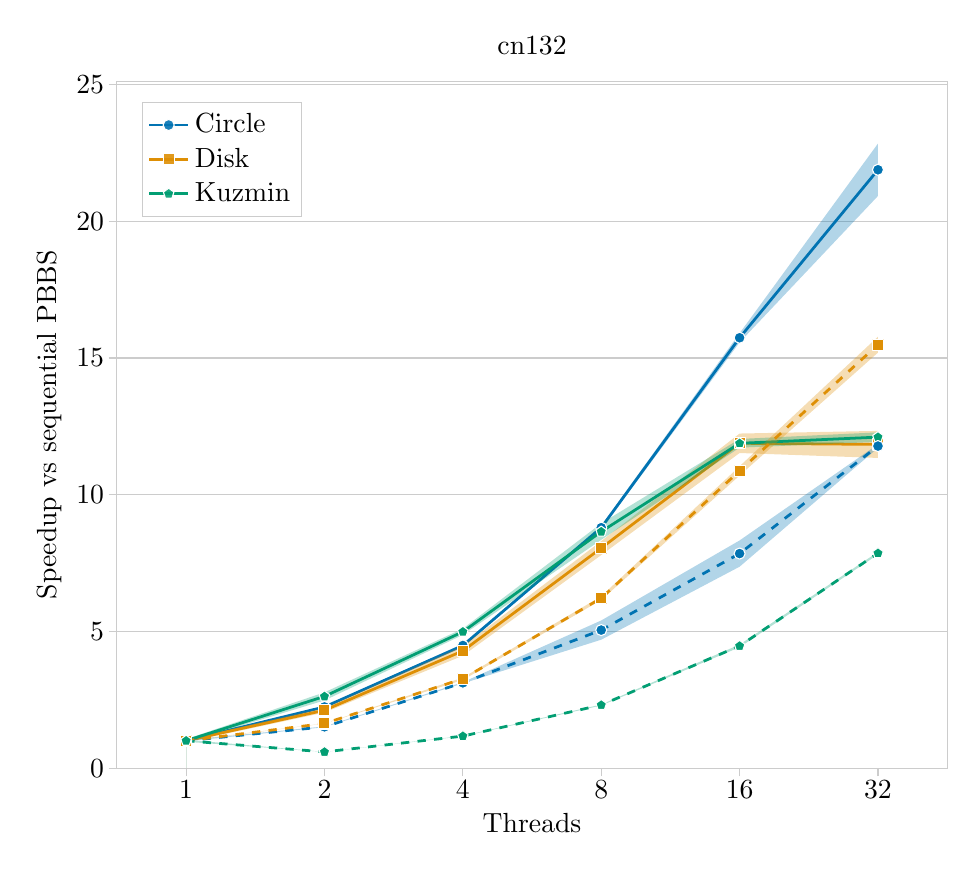
\begin{tikzpicture}
\begin{axis}[
  title={cn132},
  width=\epyfigurewidth,
  height={\epyheightratio*\epyfigurewidth},
  ymin=0,
  xlabel={Threads},
  ylabel={Speedup vs sequential PBBS},
  xmode=log,
  scaled ticks=false,
  xtick={1,2,4,8,16,32},
  extra y ticks={\pgfkeysvalueof{/pgfplots/ymax}},
  xticklabels={1,2,4,8,16,32},
  extra y tick labels={\vphantom{Ag}},
  tick pos=left,
  tick align=outside,
  ymajorgrids,
  legend pos=north west,
  legend cell align=left,
  major tick length=0.3em,
  /pgf/number format/fixed,
  axis line style={color=black!20},
  y grid style={color=black!20,line width=0.4pt},
  tick style={color=black!20,line width=0.4pt},
  tick label style={inner sep=0.15em},
  ylabel style={outer sep=-0.25em},
  extra y tick style={grid=none,major tick length=0pt,yticklabel style={opacity=0,text opacity=0}},
  legend style={draw=black!20,draw opacity=1,fill opacity=0.9,text opacity=1,inner sep=0.2em},
  legend image code/.code={\path[#1] (0em,0pt) -- (1.4em,0pt) plot coordinates {(0.7em,0pt)};},
]
\addplot[draw=none,fill=colorblind0,fill opacity=0.3,forget plot] coordinates {
  (1,1.0588324728442475)
  (2,2.255719793046268)
  (4,4.522788662370438)
  (8,8.864152208832397)
  (16,15.906419478282302)
  (32,22.842287569838273)
  (32,20.925679450832963)
  (16,15.571764509197969)
  (8,8.723853789677811)
  (4,4.446473430950995)
  (2,2.220442833900802)
  (1,0.9472076021878847)
} \closedcycle;
\addplot[color=colorblind0,line width=1pt,mark=*,mark size=2pt,mark options={draw=white,line width=-0.4pt,solid}] coordinates {
  (1,1.003020037516066)
  (2,2.238081313473535)
  (4,4.484631046660716)
  (8,8.794002999255104)
  (16,15.739091993740136)
  (32,21.883983510335618)
};
\addlegendentry{Circle}
\addplot[draw=none,fill=colorblind1,fill opacity=0.3,forget plot] coordinates {
  (1,1.05973764288434)
  (2,2.1992019809147805)
  (4,4.46458038924002)
  (8,8.304062155136563)
  (16,12.237055956899832)
  (32,12.333819211546203)
  (32,11.344433373482595)
  (16,11.524851052811583)
  (8,7.792789887037375)
  (4,4.110943714972264)
  (2,2.032950391387073)
  (1,0.9465993580303315)
} \closedcycle;
\addplot[color=colorblind1,line width=1pt,mark=square*,mark size=2pt,mark options={draw=white,line width=-0.4pt,solid}] coordinates {
  (1,1.0031685004573356)
  (2,2.1160761861509267)
  (4,4.287762052106142)
  (8,8.04842602108697)
  (16,11.880953504855707)
  (32,11.839126292514399)
};
\addlegendentry{Disk}
\addplot[draw=none,fill=colorblind2,fill opacity=0.3,forget plot] coordinates {
  (1,1.0587238312198342)
  (2,2.7720500772653636)
  (4,5.101161715804618)
  (8,8.952448782392416)
  (16,12.038325634957486)
  (32,12.280051420872798)
  (32,11.932176721229066)
  (16,11.721339375464987)
  (8,8.350136396259757)
  (4,4.872435336132249)
  (2,2.4754539905505406)
  (1,0.9468540617579133)
} \closedcycle;
\addplot[color=colorblind2,line width=1pt,mark=pentagon*,mark size=2pt,mark options={draw=white,line width=-0.4pt,solid}] coordinates {
  (1,1.0027889464888737)
  (2,2.623752033907952)
  (4,4.9867985259684335)
  (8,8.651292589326086)
  (16,11.879832505211237)
  (32,12.106114071050932)
};
\addlegendentry{Kuzmin}
\addplot[draw=none,fill=colorblind0,fill opacity=0.3,forget plot] coordinates {
  (1,1.0236006286978019)
  (2,1.5254131922657415)
  (4,3.142300855267663)
  (8,5.400616687984472)
  (16,8.327034742077359)
  (32,11.843922981041187)
  (32,11.71384687783612)
  (16,7.366683087636766)
  (8,4.6971161686486305)
  (4,3.097368978542853)
  (2,1.4961850050992074)
  (1,0.977505361538901)
} \closedcycle;
\addplot[color=colorblind0,line width=1pt,dashed,mark=*,mark size=2pt,mark options={draw=white,line width=-0.4pt,solid}] coordinates {
  (1,1.0005529951183514)
  (2,1.5107990986824744)
  (4,3.119834916905258)
  (8,5.048866428316551)
  (16,7.846858914857062)
  (32,11.778884929438654)
};
\addplot[draw=none,fill=colorblind1,fill opacity=0.3,forget plot] coordinates {
  (1,1.009316545381855)
  (2,1.635949814144872)
  (4,3.3117294522782075)
  (8,6.284162908623002)
  (16,11.042232152605303)
  (32,15.77989447541947)
  (32,15.19689062735735)
  (16,10.701398910016072)
  (8,6.146907572446163)
  (4,3.2233180229831495)
  (2,1.6301352312543118)
  (1,0.9908462805386735)
} \closedcycle;
\addplot[color=colorblind1,line width=1pt,dashed,mark=square*,mark size=2pt,mark options={draw=white,line width=-0.4pt,solid}] coordinates {
  (1,1.0000814129602642)
  (2,1.633042522699592)
  (4,3.2675237376306785)
  (8,6.2155352405345825)
  (16,10.871815531310688)
  (32,15.48839255138841)
};
\addplot[draw=none,fill=colorblind2,fill opacity=0.3,forget plot] coordinates {
  (1,1.0387734110497289)
  (2,0.5933342766421352)
  (4,1.1791447350873474)
  (8,2.326375588462051)
  (16,4.518503104035234)
  (32,7.906297255061239)
  (32,7.813438730493318)
  (16,4.420751035102811)
  (8,2.289919061114432)
  (4,1.163069535891835)
  (2,0.5922320045558958)
  (1,0.9641869873942398)
} \closedcycle;
\addplot[color=colorblind2,line width=1pt,dashed,mark=pentagon*,mark size=2pt,mark options={draw=white,line width=-0.4pt,solid}] coordinates {
  (1,1.0014801992219844)
  (2,0.5927831405990155)
  (4,1.1711071354895912)
  (8,2.3081473247882416)
  (16,4.469627069569023)
  (32,7.8598679927772785)
};
\end{axis}
\end{tikzpicture}%
  \end{subfigure}%
  \begin{subfigure}{.333\linewidth}
    \centering
    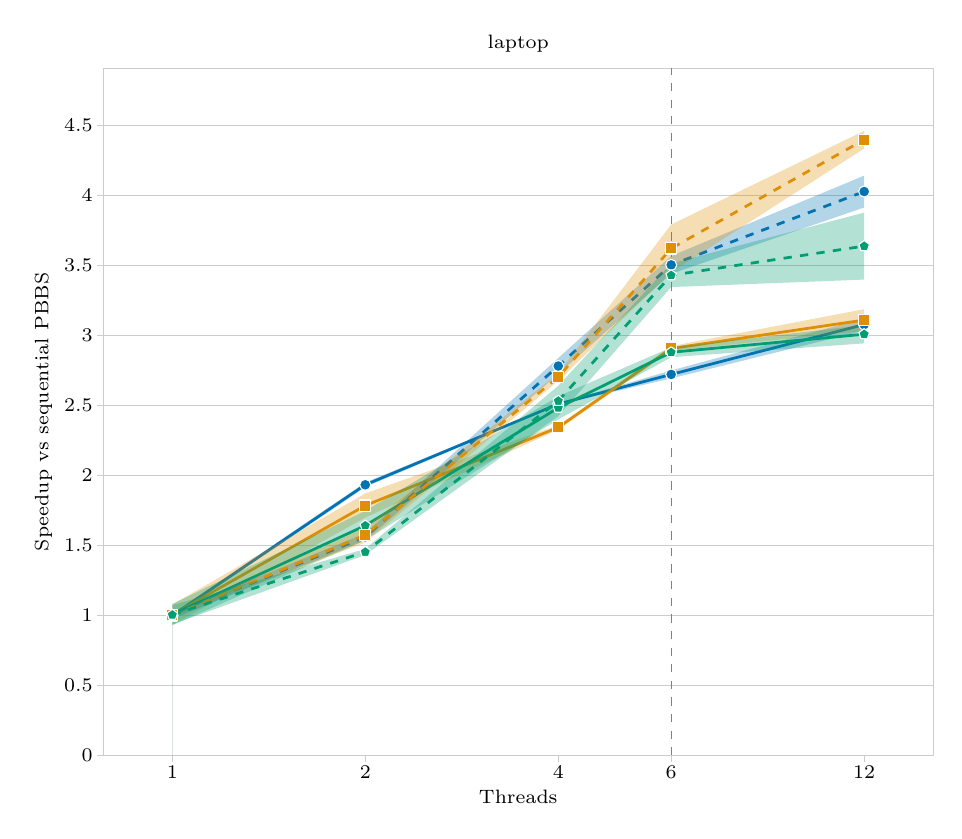
\begin{tikzpicture}
\scriptsize
\begin{axis}[
  title={laptop},
  width=\epyfigurewidth,
  height={\epyheightratio*\epyfigurewidth},
  ymin=0,
  xlabel={Threads},
  ylabel={Speedup vs sequential PBBS},
  xmode=log,
  scaled ticks=false,
  xtick={1,2,4,6,12},
  extra y ticks={\pgfkeysvalueof{/pgfplots/ymax}},
  xticklabels={1,2,4,6,12},
  extra y tick labels={\vphantom{Ag}},
  tick pos=left,
  tick align=outside,
  ymajorgrids,
  legend cell align=left,
  major tick length=0.3em,
  /pgf/number format/fixed,
  axis line style={color=black!20},
  y grid style={color=black!20,line width=0.4pt},
  title style={yshift=-1ex},
  tick style={color=black!20,line width=0.4pt},
  tick label style={inner sep=0.15em},
  ylabel style={outer sep=-0.25em},
  extra y tick style={grid=none,major tick length=0pt,yticklabel style={opacity=0,text opacity=0}},
  legend style={draw=black!20,draw opacity=1,fill opacity=0.9,text opacity=1,inner sep=0.2em},
  legend image code/.code={\path[#1] (0em,0pt) -- (1.4em,0pt) plot coordinates {(0.7em,0pt)};},
]
\addplot[draw=none,fill=colorblind0,fill opacity=0.3,forget plot] coordinates {
  (1,1.0131164581502765)
  (2,1.9501988299905444)
  (4,2.515196268099189)
  (6,2.750703820958493)
  (12,3.1219386122226456)
  (12,3.035288809149917)
  (6,2.693680013148807)
  (4,2.506742674894182)
  (2,1.9169011104317766)
  (1,0.9872052343318499)
} \closedcycle;
\addplot[color=colorblind0,line width=1pt,mark=*,mark size=2pt,mark options={draw=white,line width=-0.4pt,solid}] coordinates {
  (1,1.0001608462410632)
  (2,1.9335499702111605)
  (4,2.5109694714966855)
  (6,2.72219191705365)
  (12,3.078613710686281)
};
\addplot[draw=none,fill=colorblind1,fill opacity=0.3,forget plot] coordinates {
  (1,1.0784366031980255)
  (2,1.8717090460007038)
  (4,2.35961993380977)
  (6,2.924286106846873)
  (12,3.1886348476749684)
  (12,3.0328496094715134)
  (6,2.890861201277035)
  (4,2.327439166775244)
  (2,1.6992076934294493)
  (1,0.9320522338210531)
} \closedcycle;
\addplot[color=colorblind1,line width=1pt,mark=square*,mark size=2pt,mark options={draw=white,line width=-0.4pt,solid}] coordinates {
  (1,1.0052444185095393)
  (2,1.7854583697150765)
  (4,2.343529550292507)
  (6,2.907573654061954)
  (12,3.110742228573241)
};
\addplot[draw=none,fill=colorblind2,fill opacity=0.3,forget plot] coordinates {
  (1,1.0823447994323898)
  (2,1.7471152735663114)
  (4,2.5663994261464755)
  (6,2.915081263345394)
  (12,3.074694426870031)
  (12,2.9442609069295225)
  (6,2.8453577783863926)
  (4,2.4009814061057706)
  (2,1.5373950312097957)
  (1,0.9297076764608552)
} \closedcycle;
\addplot[color=colorblind2,line width=1pt,mark=pentagon*,mark size=2pt,mark options={draw=white,line width=-0.4pt,solid}] coordinates {
  (1,1.0060262379466225)
  (2,1.6422551523880535)
  (4,2.483690416126123)
  (6,2.8802195208658934)
  (12,3.0094776668997767)
};
\addplot[draw=none,fill=colorblind0,fill opacity=0.3,forget plot] coordinates {
  (1,1.0252585436377575)
  (2,1.5866906110955716)
  (4,2.8393403575581027)
  (6,3.5684211941858885)
  (12,4.142550650216816)
  (12,3.9150281740577464)
  (6,3.4412260636229854)
  (4,2.7253896497907104)
  (2,1.537360284471817)
  (1,0.9759355598930046)
} \closedcycle;
\addplot[color=colorblind0,line width=1pt,dashed,mark=*,mark size=2pt,mark options={draw=white,line width=-0.4pt,solid}] coordinates {
  (1,1.000597051765381)
  (2,1.5620254477836943)
  (4,2.7823650036744065)
  (6,3.504823628904437)
  (12,4.028789412137281)
};
\addplot[draw=none,fill=colorblind1,fill opacity=0.3,forget plot] coordinates {
  (1,1.0067955765168013)
  (2,1.6279631332995335)
  (4,2.7308323435452393)
  (6,3.7931776652712017)
  (12,4.462347314705178)
  (12,4.336159571563273)
  (6,3.4511531241215456)
  (4,2.677138186424149)
  (2,1.5209952154179036)
  (1,0.99329182315633)
} \closedcycle;
\addplot[color=colorblind1,line width=1pt,dashed,mark=square*,mark size=2pt,mark options={draw=white,line width=-0.4pt,solid}] coordinates {
  (1,1.0000436998365656)
  (2,1.5744791743587185)
  (4,2.703985264984694)
  (6,3.6221653946963737)
  (12,4.399253443134225)
};
\addplot[draw=none,fill=colorblind2,fill opacity=0.3,forget plot] coordinates {
  (1,1.072801312951939)
  (2,1.4757146130285748)
  (4,2.641268566195949)
  (6,3.515097560831859)
  (12,3.878519396630166)
  (12,3.3997730701545947)
  (6,3.3461422048369647)
  (4,2.4246004898027023)
  (2,1.4319847420148684)
  (1,0.936702732693216)
} \closedcycle;
\addplot[color=colorblind2,line width=1pt,dashed,mark=pentagon*,mark size=2pt,mark options={draw=white,line width=-0.4pt,solid}] coordinates {
  (1,1.0047520228225775)
  (2,1.4538496775217216)
  (4,2.5329345279993256)
  (6,3.430619882834412)
  (12,3.6391462333923803)
};
\draw[draw=gray,dashed] (axis cs:6,0) -- (axis cs:6,30);
\end{axis}%
\end{tikzpicture}%%
  \end{subfigure}%
  \caption{Speedup for $10^8$ points, compared to each sequential
  implementation. The solid lines represent the VQhull implementation, the
  dashed lines represent the PBBS implementation.}
\end{figure}

\begin{figure}
  \scriptsize
  \begin{subfigure}{.333\linewidth}
    \centering
    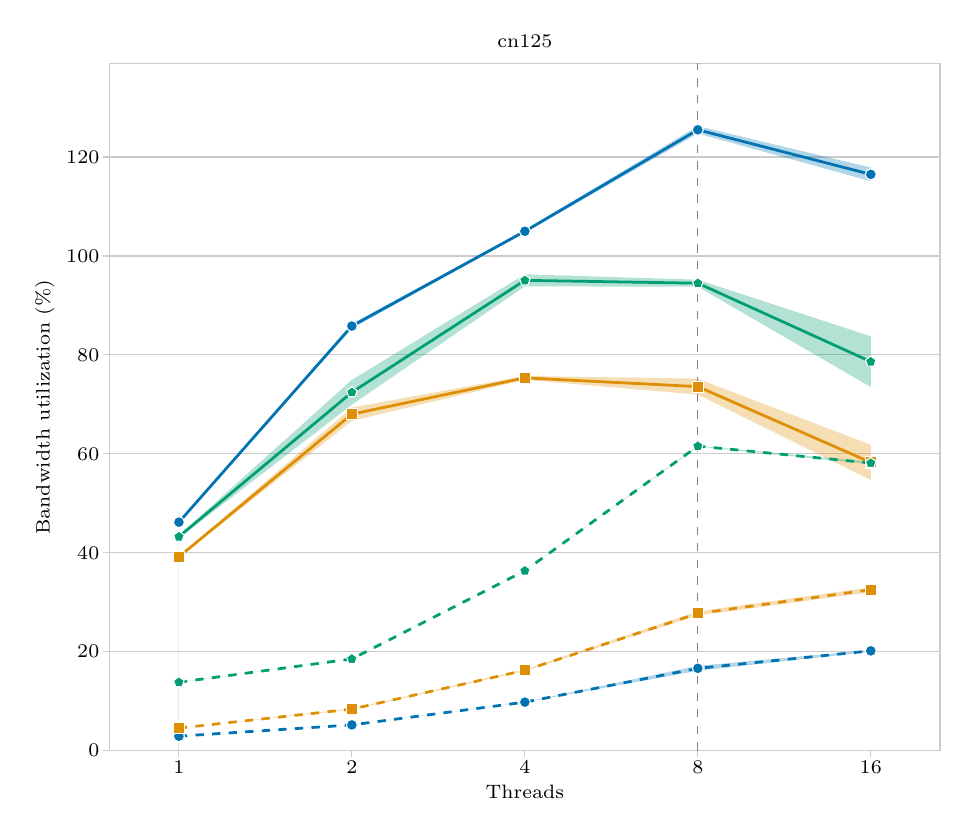
\begin{tikzpicture}
\scriptsize
\begin{axis}[
  title={cn125},
  width=\epyfigurewidth,
  height={\epyheightratio*\epyfigurewidth},
  ymin=0,
  xlabel={Threads},
  ylabel={Bandwidth utilization (\si{{\percent}})},
  xmode=log,
  scaled ticks=false,
  xtick={1,2,4,8,16},
  extra y ticks={\pgfkeysvalueof{/pgfplots/ymax}},
  xticklabels={1,2,4,8,16},
  extra y tick labels={\vphantom{Ag}},
  tick pos=left,
  tick align=outside,
  ymajorgrids,
  legend cell align=left,
  major tick length=0.3em,
  /pgf/number format/fixed,
  axis line style={color=black!20},
  y grid style={color=black!20,line width=0.4pt},
  title style={yshift=-1ex},
  tick style={color=black!20,line width=0.4pt},
  tick label style={inner sep=0.15em},
  ylabel style={outer sep=-0.25em},
  extra y tick style={grid=none,major tick length=0pt,yticklabel style={opacity=0,text opacity=0}},
  legend style={draw=black!20,draw opacity=1,fill opacity=0.9,text opacity=1,inner sep=0.2em},
  legend image code/.code={\path[#1] (0em,0pt) -- (1.4em,0pt) plot coordinates {(0.7em,0pt)};},
]
\addplot[draw=none,fill=colorblind0,fill opacity=0.3,forget plot] coordinates {
  (1,46.32527327850714)
  (2,86.30472676434194)
  (4,105.28004815016888)
  (8,126.24515408111516)
  (16,117.88035711247232)
  (16,115.11686450071878)
  (8,124.75714720088298)
  (4,104.69782388074958)
  (2,85.36927854874504)
  (1,46.05686541820134)
} \closedcycle;
\addplot[color=colorblind0,line width=1pt,mark=*,mark size=2pt,mark options={draw=white,line width=-0.4pt,solid}] coordinates {
  (1,46.19106934835424)
  (2,85.83700265654349)
  (4,104.98893601545923)
  (8,125.50115064099907)
  (16,116.49861080659555)
};
\addplot[draw=none,fill=colorblind1,fill opacity=0.3,forget plot] coordinates {
  (1,39.35251415929797)
  (2,69.37530093535898)
  (4,75.74958221214688)
  (8,75.20095008946606)
  (16,61.838755897228474)
  (16,54.701507698108564)
  (8,71.98791064869215)
  (4,74.97440956700056)
  (2,66.66649524311939)
  (1,39.03017055887322)
} \closedcycle;
\addplot[color=colorblind1,line width=1pt,mark=square*,mark size=2pt,mark options={draw=white,line width=-0.4pt,solid}] coordinates {
  (1,39.191342359085596)
  (2,68.02089808923918)
  (4,75.36199588957372)
  (8,73.5944303690791)
  (16,58.27013179766852)
};
\addplot[draw=none,fill=colorblind2,fill opacity=0.3,forget plot] coordinates {
  (1,43.56690382578265)
  (2,74.95086511429379)
  (4,96.29326605440836)
  (8,95.2048642241951)
  (16,83.76381729730926)
  (16,73.51612190327805)
  (8,93.78714675140837)
  (4,93.85533076948396)
  (2,69.9448398840784)
  (1,42.96333964950018)
} \closedcycle;
\addplot[color=colorblind2,line width=1pt,mark=pentagon*,mark size=2pt,mark options={draw=white,line width=-0.4pt,solid}] coordinates {
  (1,43.265121737641415)
  (2,72.4478524991861)
  (4,95.07429841194616)
  (8,94.49600548780174)
  (16,78.63996960029365)
};
\addplot[draw=none,fill=colorblind0,fill opacity=0.3,forget plot] coordinates {
  (1,2.9357214815409285)
  (2,5.218864038228963)
  (4,9.84013686348858)
  (8,17.1412918380299)
  (16,20.334820966366696)
  (16,20.0228486758017)
  (8,16.154447274183333)
  (4,9.784176760300136)
  (2,5.205145190618312)
  (1,2.925599187296488)
} \closedcycle;
\addplot[color=colorblind0,line width=1pt,dashed,mark=*,mark size=2pt,mark options={draw=white,line width=-0.4pt,solid}] coordinates {
  (1,2.9306603344187083)
  (2,5.212004614423638)
  (4,9.812156811894358)
  (8,16.647869556106617)
  (16,20.178834821084198)
};
\addplot[draw=none,fill=colorblind1,fill opacity=0.3,forget plot] coordinates {
  (1,4.570274043709936)
  (2,8.503817467480072)
  (4,16.4110097609223)
  (8,28.150077997815853)
  (16,33.01474067274618)
  (16,32.058905676870204)
  (8,27.326770181890634)
  (4,16.076335477716338)
  (2,8.312827299194584)
  (1,4.560484619364467)
} \closedcycle;
\addplot[color=colorblind1,line width=1pt,dashed,mark=square*,mark size=2pt,mark options={draw=white,line width=-0.4pt,solid}] coordinates {
  (1,4.565379331537201)
  (2,8.408322383337328)
  (4,16.24367261931932)
  (8,27.738424089853243)
  (16,32.53682317480819)
};
\addplot[draw=none,fill=colorblind2,fill opacity=0.3,forget plot] coordinates {
  (1,13.861888698424476)
  (2,18.552236446261553)
  (4,36.38464536396844)
  (8,61.658416155588235)
  (16,58.39593927896554)
  (16,57.90337361992552)
  (8,61.47885097651169)
  (4,36.3572696085591)
  (2,18.54191481498558)
  (1,13.819019617298242)
} \closedcycle;
\addplot[color=colorblind2,line width=1pt,dashed,mark=pentagon*,mark size=2pt,mark options={draw=white,line width=-0.4pt,solid}] coordinates {
  (1,13.840454157861359)
  (2,18.547075630623567)
  (4,36.37095748626377)
  (8,61.56863356604996)
  (16,58.14965644944553)
};
\draw[draw=gray,dashed] (axis cs:8,0) -- (axis cs:8,200);
\end{axis}%
\end{tikzpicture}%%
  \end{subfigure}%
  \begin{subfigure}{.333\linewidth}
    \centering
    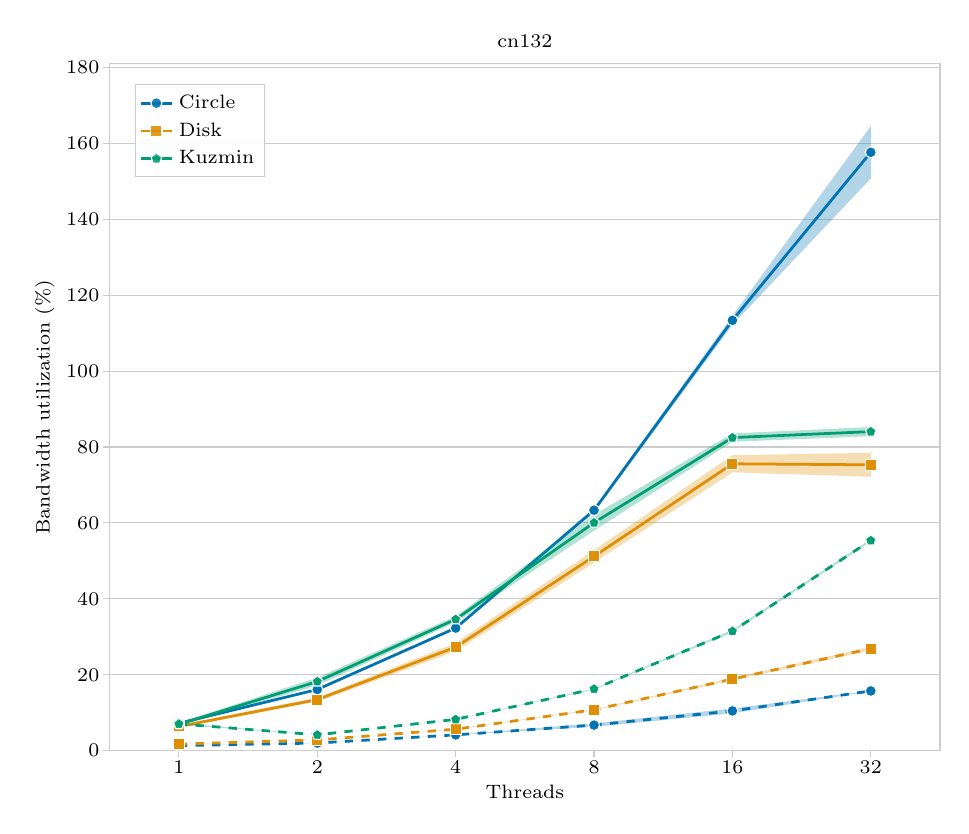
\begin{tikzpicture}
\scriptsize
\begin{axis}[
  title={cn132},
  width=\epyfigurewidth,
  height={\epyheightratio*\epyfigurewidth},
  ymin=0,
  xlabel={Threads},
  ylabel={Bandwidth utilization (\si{{\percent}})},
  xmode=log,
  scaled ticks=false,
  xtick={1,2,4,8,16,32},
  extra y ticks={\pgfkeysvalueof{/pgfplots/ymax}},
  xticklabels={1,2,4,8,16,32},
  extra y tick labels={\vphantom{Ag}},
  tick pos=left,
  tick align=outside,
  ymajorgrids,
  legend pos=north west,
  legend cell align=left,
  major tick length=0.3em,
  /pgf/number format/fixed,
  axis line style={color=black!20},
  y grid style={color=black!20,line width=0.4pt},
  title style={yshift=-1ex},
  tick style={color=black!20,line width=0.4pt},
  tick label style={inner sep=0.15em},
  ylabel style={outer sep=-0.25em},
  extra y tick style={grid=none,major tick length=0pt,yticklabel style={opacity=0,text opacity=0}},
  legend style={draw=black!20,draw opacity=1,fill opacity=0.9,text opacity=1,inner sep=0.2em},
  legend image code/.code={\path[#1] (0em,0pt) -- (1.4em,0pt) plot coordinates {(0.7em,0pt)};},
]
\addplot[draw=none,fill=colorblind0,fill opacity=0.3,forget plot] coordinates {
  (1,7.627070022392399)
  (2,16.248588189069583)
  (4,32.57892698711748)
  (8,63.85099750888911)
  (16,114.57844208396448)
  (32,164.53946326257736)
  (32,150.73359245293742)
  (16,112.16782761188337)
  (8,62.840388281870815)
  (4,32.029206772882226)
  (2,15.994478266603007)
  (1,6.823004481741183)
} \closedcycle;
\addplot[color=colorblind0,line width=1pt,mark=*,mark size=2pt,mark options={draw=white,line width=-0.4pt,solid}] coordinates {
  (1,7.225037252066791)
  (2,16.121533227836295)
  (4,32.30406687999985)
  (8,63.34569289537996)
  (16,113.37313484792392)
  (32,157.6365278577574)
};
\addlegendentry{Circle}
\addplot[draw=none,fill=colorblind1,fill opacity=0.3,forget plot] coordinates {
  (1,6.741636665289068)
  (2,13.990463402392864)
  (4,28.401915369647803)
  (8,52.8271976293457)
  (16,77.8473669102587)
  (32,78.46293691454876)
  (32,72.16885093317974)
  (16,73.3165976893676)
  (8,49.574683300250406)
  (4,26.152217073619084)
  (2,12.932835772433412)
  (1,6.021895119311969)
} \closedcycle;
\addplot[color=colorblind1,line width=1pt,mark=square*,mark size=2pt,mark options={draw=white,line width=-0.4pt,solid}] coordinates {
  (1,6.3817658923005185)
  (2,13.461649587413138)
  (4,27.277066221633444)
  (8,51.20094046479805)
  (16,75.58198229981315)
  (32,75.31589392386425)
};
\addlegendentry{Disk}
\addplot[draw=none,fill=colorblind2,fill opacity=0.3,forget plot] coordinates {
  (1,7.351268020715182)
  (2,19.24777971734405)
  (4,35.42000839509254)
  (8,62.16148961648025)
  (16,83.58833120933419)
  (32,85.26675856440193)
  (32,82.85128431200846)
  (16,81.38733139833677)
  (8,57.97932269807235)
  (4,33.83184265177293)
  (2,17.188359438852924)
  (1,6.574498258403636)
} \closedcycle;
\addplot[color=colorblind2,line width=1pt,mark=pentagon*,mark size=2pt,mark options={draw=white,line width=-0.4pt,solid}] coordinates {
  (1,6.962883139559409)
  (2,18.218069578098486)
  (4,34.625925523432734)
  (8,60.0704061572763)
  (16,82.48783130383548)
  (32,84.05902143820519)
};
\addlegendentry{Kuzmin}
\addplot[draw=none,fill=colorblind0,fill opacity=0.3,forget plot] coordinates {
  (1,1.3678662352412623)
  (2,2.0384524413064926)
  (4,4.199144783995001)
  (8,7.216995583885496)
  (16,11.127650124501148)
  (32,15.827366537645291)
  (32,15.65354219190185)
  (16,9.844305267885986)
  (8,6.276888104566734)
  (4,4.13910105665177)
  (2,1.9993939948562638)
  (1,1.306267836624314)
} \closedcycle;
\addplot[color=colorblind0,line width=1pt,dashed,mark=*,mark size=2pt,mark options={draw=white,line width=-0.4pt,solid}] coordinates {
  (1,1.337067035932788)
  (2,2.0189232180813783)
  (4,4.169122920323385)
  (8,6.746941844226115)
  (16,10.485977696193567)
  (32,15.740454364773571)
};
\addplot[draw=none,fill=colorblind1,fill opacity=0.3,forget plot] coordinates {
  (1,1.751581062302018)
  (2,2.8390485883183048)
  (4,5.747218371302671)
  (8,10.90561805761388)
  (16,19.162833317795734)
  (32,27.384634141523986)
  (32,26.372881679734636)
  (16,18.57134687496087)
  (8,10.66742336176027)
  (4,5.593788026825668)
  (2,2.828957885532453)
  (1,1.7195275244272579)
} \closedcycle;
\addplot[color=colorblind1,line width=1pt,dashed,mark=square*,mark size=2pt,mark options={draw=white,line width=-0.4pt,solid}] coordinates {
  (1,1.735554293364638)
  (2,2.834003236925379)
  (4,5.67050319906417)
  (8,10.786520709687075)
  (16,18.867090096378302)
  (32,26.87875791062931)
};
\addplot[draw=none,fill=colorblind2,fill opacity=0.3,forget plot] coordinates {
  (1,7.319400323330377)
  (2,4.1807491894779885)
  (4,8.308484086563196)
  (8,16.392096729901645)
  (16,31.838255320015612)
  (32,55.709314533341406)
  (32,55.05501523426752)
  (16,31.149475151656134)
  (8,16.13521691836891)
  (4,8.195215093597414)
  (2,4.172982365088186)
  (1,6.793849815767463)
} \closedcycle;
\addplot[color=colorblind2,line width=1pt,dashed,mark=pentagon*,mark size=2pt,mark options={draw=white,line width=-0.4pt,solid}] coordinates {
  (1,7.05662506954892)
  (2,4.176865777283087)
  (4,8.251849590080305)
  (8,16.26365682413528)
  (16,31.493865235835873)
  (32,55.382164883804464)
};
\end{axis}%
\end{tikzpicture}%%
  \end{subfigure}%
  \begin{subfigure}{.333\linewidth}
    \centering
    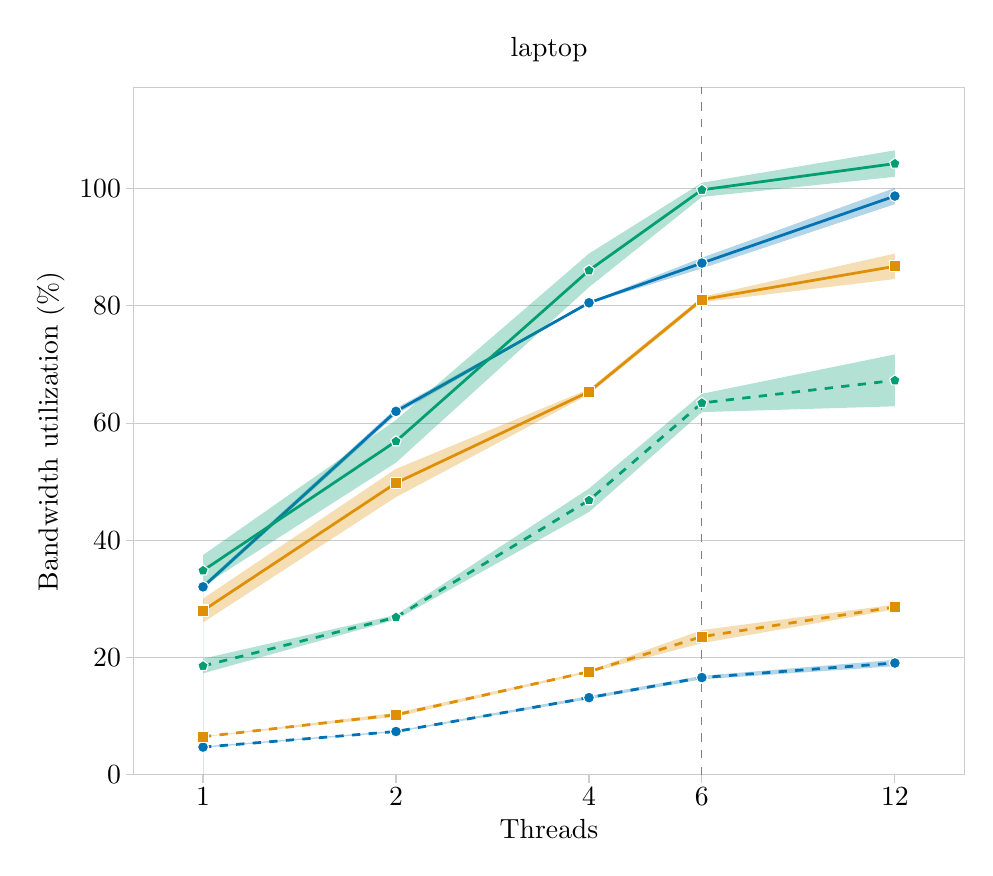
\begin{tikzpicture}
\begin{axis}[
  title={laptop},
  width=\epyfigurewidth,
  height={\epyheightratio*\epyfigurewidth},
  ymin=0,
  xlabel={Threads},
  ylabel={Bandwidth utilization (\si{{\percent}})},
  xmode=log,
  scaled ticks=false,
  xtick={1,2,4,6,12},
  extra y ticks={\pgfkeysvalueof{/pgfplots/ymax}},
  xticklabels={1,2,4,6,12},
  extra y tick labels={\vphantom{Ag}},
  tick pos=left,
  tick align=outside,
  ymajorgrids,
  legend cell align=left,
  major tick length=0.3em,
  /pgf/number format/fixed,
  axis line style={color=black!20},
  y grid style={color=black!20,line width=0.4pt},
  tick style={color=black!20,line width=0.4pt},
  tick label style={inner sep=0.15em},
  ylabel style={outer sep=-0.25em},
  extra y tick style={grid=none,major tick length=0pt,yticklabel style={opacity=0,text opacity=0}},
  legend style={draw=black!20,draw opacity=1,fill opacity=0.9,text opacity=1,inner sep=0.2em},
  legend image code/.code={\path[#1] (0em,0pt) -- (1.4em,0pt) plot coordinates {(0.7em,0pt)};},
]
\addplot[draw=none,fill=colorblind0,fill opacity=0.3,forget plot] coordinates {
  (1,32.484831403554885)
  (2,62.53168595377395)
  (4,80.64791175659012)
  (6,88.1992876002579)
  (12,100.10265715696993)
  (12,97.32429518157763)
  (6,86.37086129468939)
  (4,80.37685353045067)
  (2,61.46401915467336)
  (1,31.65400713806209)
} \closedcycle;
\addplot[color=colorblind0,line width=1pt,mark=*,mark size=2pt,mark options={draw=white,line width=-0.4pt,solid}] coordinates {
  (1,32.06941927080849)
  (2,61.997852554223655)
  (4,80.5123826435204)
  (6,87.28507444747365)
  (12,98.71347616927378)
};
\addplot[draw=none,fill=colorblind1,fill opacity=0.3,forget plot] coordinates {
  (1,30.06856681795748)
  (2,52.18629296015595)
  (4,65.79004220957009)
  (6,81.53385367095537)
  (12,88.90432658819644)
  (12,84.56078072719613)
  (6,80.60191293050737)
  (4,64.89279007535902)
  (2,47.37667463804455)
  (1,25.98713247247669)
} \closedcycle;
\addplot[color=colorblind1,line width=1pt,mark=square*,mark size=2pt,mark options={draw=white,line width=-0.4pt,solid}] coordinates {
  (1,28.027849645217085)
  (2,49.78148379910025)
  (4,65.34141614246455)
  (6,81.06788330073137)
  (12,86.73255365769629)
};
\addplot[draw=none,fill=colorblind2,fill opacity=0.3,forget plot] coordinates {
  (1,37.49361584187408)
  (2,60.52199717956696)
  (4,88.90290250500976)
  (6,100.98162534992127)
  (12,106.51080111686483)
  (12,101.99244033930344)
  (6,98.56632704426079)
  (4,83.17264011544393)
  (2,53.25705701881265)
  (1,32.20609780242412)
} \closedcycle;
\addplot[color=colorblind2,line width=1pt,mark=pentagon*,mark size=2pt,mark options={draw=white,line width=-0.4pt,solid}] coordinates {
  (1,34.8498568221491)
  (2,56.889527099189806)
  (4,86.03777131022684)
  (6,99.77397619709103)
  (12,104.25162072808413)
};
\addplot[draw=none,fill=colorblind0,fill opacity=0.3,forget plot] coordinates {
  (1,4.85523253740951)
  (2,7.513960190431021)
  (4,13.446030539655544)
  (6,16.89867867642413)
  (12,19.617536307901187)
  (12,18.540076835756768)
  (6,16.296331160920513)
  (4,12.906403547570159)
  (2,7.280350621029262)
  (1,4.621657741075744)
} \closedcycle;
\addplot[color=colorblind0,line width=1pt,dashed,mark=*,mark size=2pt,mark options={draw=white,line width=-0.4pt,solid}] coordinates {
  (1,4.738445139242627)
  (2,7.397155405730142)
  (4,13.176217043612851)
  (6,16.59750491867232)
  (12,19.078806571828977)
};
\addplot[draw=none,fill=colorblind1,fill opacity=0.3,forget plot] coordinates {
  (1,6.553032530990638)
  (2,10.596088839279147)
  (4,17.774445578957824)
  (6,24.689040373365692)
  (12,29.04453277298816)
  (12,28.2232018046082)
  (6,22.462870536282153)
  (4,17.42496097002067)
  (2,9.899855897855453)
  (1,6.465139281233032)
} \closedcycle;
\addplot[color=colorblind1,line width=1pt,dashed,mark=square*,mark size=2pt,mark options={draw=white,line width=-0.4pt,solid}] coordinates {
  (1,6.509085906111835)
  (2,10.2479723685673)
  (4,17.599703274489247)
  (6,23.575955454823923)
  (12,28.63386728879818)
};
\addplot[draw=none,fill=colorblind2,fill opacity=0.3,forget plot] coordinates {
  (1,19.834586367531553)
  (2,27.28388620759916)
  (4,48.83333834846525)
  (6,64.98920659294762)
  (12,71.70836484057673)
  (12,62.85701907321416)
  (6,61.86545985598971)
  (4,44.82745056437628)
  (2,26.475382439948348)
  (1,17.318315169827496)
} \closedcycle;
\addplot[color=colorblind2,line width=1pt,dashed,mark=pentagon*,mark size=2pt,mark options={draw=white,line width=-0.4pt,solid}] coordinates {
  (1,18.576450768679525)
  (2,26.879634323773754)
  (4,46.83039445642076)
  (6,63.42733322446867)
  (12,67.28269195689545)
};
\draw[draw=gray,dashed] (axis cs:6,0) -- (axis cs:6,200);
\end{axis}
\end{tikzpicture}%
  \end{subfigure}%
  \caption{Bandwidth utilization for $10^8$ points, as a percentage of STREAM's
  bandwidth. The solid lines represent the VQhull implementation, the dashed
  lines represent the PBBS implementation.}%
\end{figure}

\begin{figure}
  \scriptsize
  \begin{subfigure}{.333\linewidth}
    \centering
    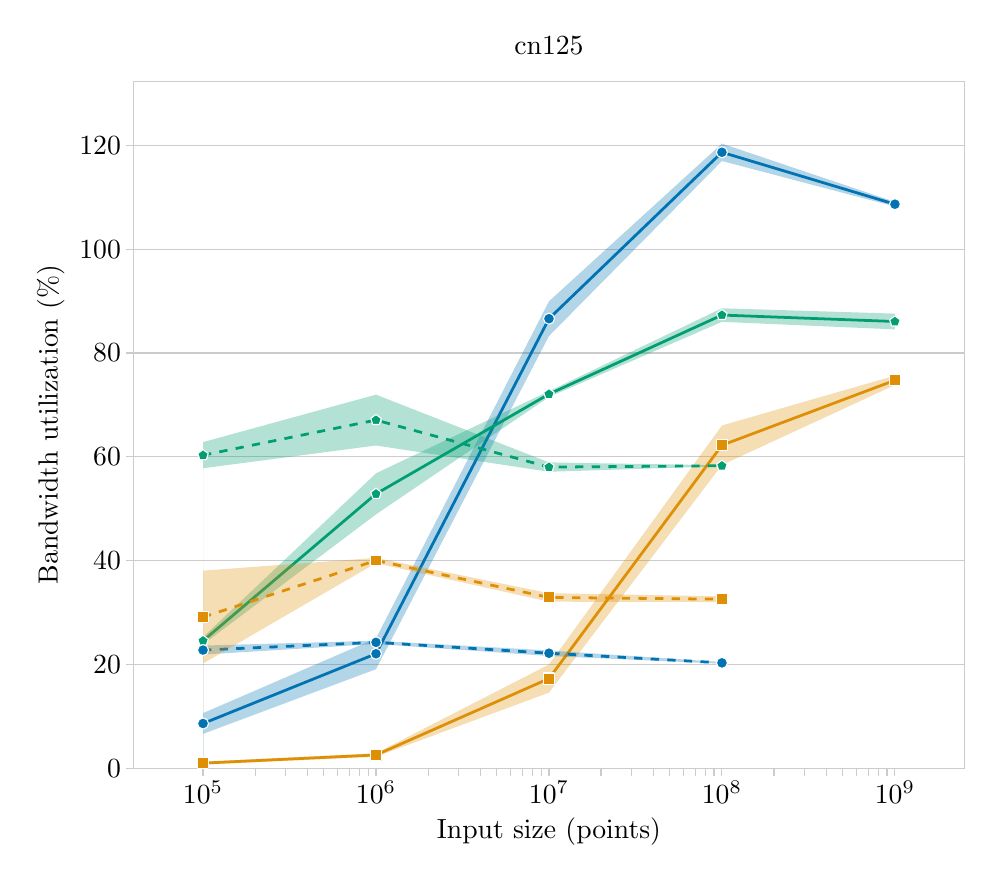
\begin{tikzpicture}
\begin{axis}[
  title={cn125},
  width=\epyfigurewidth,
  height={\epyheightratio*\epyfigurewidth},
  ymin=0,
  xlabel={Input size (points)},
  ylabel={Bandwidth utilization (\si{{\percent}})},
  xmode=log,
  scaled ticks=false,
  xtick={100000,1000000,10000000,100000000,1000000000},
  extra y ticks={\pgfkeysvalueof{/pgfplots/ymax}},
  extra y tick labels={\vphantom{Ag}},
  tick pos=left,
  tick align=outside,
  ymajorgrids,
  legend cell align=left,
  major tick length=0.3em,
  /pgf/number format/fixed,
  axis line style={color=black!20},
  y grid style={color=black!20,line width=0.4pt},
  tick style={color=black!20,line width=0.4pt},
  tick label style={inner sep=0.15em},
  ylabel style={outer sep=-0.25em},
  extra y tick style={grid=none,major tick length=0pt,yticklabel style={opacity=0,text opacity=0}},
  legend style={draw=black!20,draw opacity=1,fill opacity=0.9,text opacity=1,inner sep=0.2em},
  legend image code/.code={\path[#1] (0em,0pt) -- (1.4em,0pt) plot coordinates {(0.7em,0pt)};},
]
\addplot[draw=none,fill=colorblind0,fill opacity=0.3,forget plot] coordinates {
  (100000,10.59838990844274)
  (1000000,25.010175164791637)
  (10000000,89.95762076662604)
  (100000000,120.3579674290643)
  (1000000000,109.11645092804427)
  (1000000000,108.22562906086766)
  (100000000,116.99847889018702)
  (10000000,83.2648318699404)
  (1000000,19.069903604820308)
  (100000,6.595851787274451)
} \closedcycle;
\addplot[color=colorblind0,line width=1pt,mark=*,mark size=2pt,mark options={draw=white,line width=-0.4pt,solid}] coordinates {
  (100000,8.597120847858596)
  (1000000,22.040039384805972)
  (10000000,86.61122631828322)
  (100000000,118.67822315962566)
  (1000000000,108.67103999445597)
};
\addplot[draw=none,fill=colorblind1,fill opacity=0.3,forget plot] coordinates {
  (100000,1.244099927722852)
  (1000000,2.8712141534996802)
  (10000000,19.963637538223686)
  (100000000,66.03091200197035)
  (1000000000,75.63591453228142)
  (1000000000,73.83158460212167)
  (100000000,58.41502022480751)
  (10000000,14.547699315042292)
  (1000000,2.194960116716319)
  (100000,0.6781624185700696)
} \closedcycle;
\addplot[color=colorblind1,line width=1pt,mark=square*,mark size=2pt,mark options={draw=white,line width=-0.4pt,solid}] coordinates {
  (100000,0.9611311731464608)
  (1000000,2.5330871351079995)
  (10000000,17.25566842663299)
  (100000000,62.222966113388935)
  (1000000000,74.73374956720154)
};
\addplot[draw=none,fill=colorblind2,fill opacity=0.3,forget plot] coordinates {
  (100000,25.244977242300607)
  (1000000,56.811373815906144)
  (10000000,72.63699032045801)
  (100000000,88.61606622988985)
  (1000000000,87.58760947633269)
  (1000000000,84.54760204353414)
  (100000000,86.00195414399549)
  (10000000,71.52050682901736)
  (1000000,48.899521427069764)
  (100000,23.836124842048626)
} \closedcycle;
\addplot[color=colorblind2,line width=1pt,mark=pentagon*,mark size=2pt,mark options={draw=white,line width=-0.4pt,solid}] coordinates {
  (100000,24.540551042174616)
  (1000000,52.855447621487954)
  (10000000,72.07874857473769)
  (100000000,87.30901018694267)
  (1000000000,86.06760575993341)
};
\addplot[draw=none,fill=colorblind0,fill opacity=0.3,forget plot] coordinates {
  (100000,23.615434628003666)
  (1000000,24.54923576464996)
  (10000000,22.6768993078029)
  (100000000,20.443175950664692)
  (100000000,20.12385175961457)
  (10000000,21.610632216281395)
  (1000000,23.924392889424038)
  (100000,21.882115003443932)
} \closedcycle;
\addplot[color=colorblind0,line width=1pt,dashed,mark=*,mark size=2pt,mark options={draw=white,line width=-0.4pt,solid}] coordinates {
  (100000,22.7487748157238)
  (1000000,24.236814327037)
  (10000000,22.143765762042147)
  (100000000,20.28351385513963)
};
\addplot[draw=none,fill=colorblind1,fill opacity=0.3,forget plot] coordinates {
  (100000,38.05388026110748)
  (1000000,40.515605050606794)
  (10000000,33.71331495631996)
  (100000000,33.10200552338219)
  (100000000,32.003770952175046)
  (10000000,32.06940119329957)
  (1000000,39.50829823068375)
  (100000,20.158707817333983)
} \closedcycle;
\addplot[color=colorblind1,line width=1pt,dashed,mark=square*,mark size=2pt,mark options={draw=white,line width=-0.4pt,solid}] coordinates {
  (100000,29.10629403922073)
  (1000000,40.01195164064527)
  (10000000,32.891358074809766)
  (100000000,32.55288823777862)
};
\addplot[draw=none,fill=colorblind2,fill opacity=0.3,forget plot] coordinates {
  (100000,62.82416339617754)
  (1000000,71.9695938365408)
  (10000000,58.91256491072156)
  (100000000,58.353641083575866)
  (100000000,58.180431132609186)
  (10000000,57.10881785296495)
  (1000000,62.17532868693628)
  (100000,57.78625728904207)
} \closedcycle;
\addplot[color=colorblind2,line width=1pt,dashed,mark=pentagon*,mark size=2pt,mark options={draw=white,line width=-0.4pt,solid}] coordinates {
  (100000,60.305210342609804)
  (1000000,67.07246126173854)
  (10000000,58.01069138184325)
  (100000000,58.267036108092526)
};
\end{axis}%
\end{tikzpicture}%%
  \end{subfigure}%
  \begin{subfigure}{.333\linewidth}
    \centering
    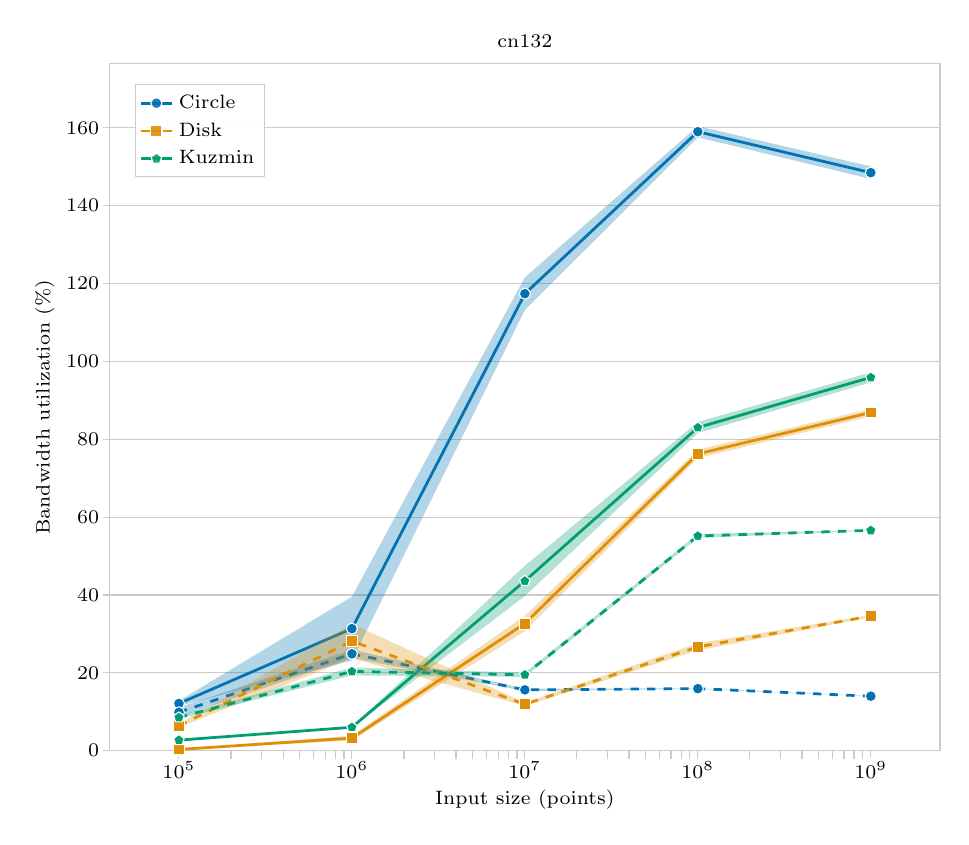
\begin{tikzpicture}
\scriptsize
\begin{axis}[
  title={cn132},
  width=\epyfigurewidth,
  height={\epyheightratio*\epyfigurewidth},
  ymin=0,
  xlabel={Input size (points)},
  ylabel={Bandwidth utilization (\si{{\percent}})},
  xmode=log,
  scaled ticks=false,
  xtick={100000,1000000,10000000,100000000,1000000000},
  extra y ticks={\pgfkeysvalueof{/pgfplots/ymax}},
  extra y tick labels={\vphantom{Ag}},
  tick pos=left,
  tick align=outside,
  ymajorgrids,
  legend pos=north west,
  legend cell align=left,
  major tick length=0.3em,
  /pgf/number format/fixed,
  axis line style={color=black!20},
  y grid style={color=black!20,line width=0.4pt},
  title style={yshift=-1ex},
  tick style={color=black!20,line width=0.4pt},
  tick label style={inner sep=0.15em},
  ylabel style={outer sep=-0.25em},
  extra y tick style={grid=none,major tick length=0pt,yticklabel style={opacity=0,text opacity=0}},
  legend style={draw=black!20,draw opacity=1,fill opacity=0.9,text opacity=1,inner sep=0.2em},
  legend image code/.code={\path[#1] (0em,0pt) -- (1.4em,0pt) plot coordinates {(0.7em,0pt)};},
]
\addplot[draw=none,fill=colorblind0,fill opacity=0.3,forget plot] coordinates {
  (100000,12.800188566628758)
  (1000000,39.55735755959984)
  (10000000,121.59097001241048)
  (100000000,160.43709207583683)
  (1000000000,150.09385663827987)
  (1000000000,146.89406603478136)
  (100000000,157.56992697288646)
  (10000000,113.1872107053401)
  (1000000,23.149847167842744)
  (100000,11.45273044325339)
} \closedcycle;
\addplot[color=colorblind0,line width=1pt,mark=*,mark size=2pt,mark options={draw=white,line width=-0.4pt,solid}] coordinates {
  (100000,12.126459504941074)
  (1000000,31.353602363721294)
  (10000000,117.3890903588753)
  (100000000,159.00350952436165)
  (1000000000,148.49396133653062)
};
\addlegendentry{Circle}
\addplot[draw=none,fill=colorblind1,fill opacity=0.3,forget plot] coordinates {
  (100000,0.3743103035411093)
  (1000000,3.853500365844502)
  (10000000,34.63895231784267)
  (100000000,77.3352493333508)
  (1000000000,87.8190987263642)
  (1000000000,85.92279759001208)
  (100000000,75.15340347369063)
  (10000000,30.69339340424941)
  (1000000,2.611455102485167)
  (100000,0.24571585409322194)
} \closedcycle;
\addplot[color=colorblind1,line width=1pt,mark=square*,mark size=2pt,mark options={draw=white,line width=-0.4pt,solid}] coordinates {
  (100000,0.3100130788171656)
  (1000000,3.2324777341648345)
  (10000000,32.66617286104604)
  (100000000,76.24432640352072)
  (1000000000,86.87094815818814)
};
\addlegendentry{Disk}
\addplot[draw=none,fill=colorblind2,fill opacity=0.3,forget plot] coordinates {
  (100000,2.8001796371518006)
  (1000000,6.119886808170244)
  (10000000,47.4925023152459)
  (100000000,84.43825988556559)
  (1000000000,97.1770573618142)
  (1000000000,94.60758333039686)
  (100000000,81.57249444600363)
  (10000000,39.71419629414042)
  (1000000,5.907336790289837)
  (100000,2.6322487405771273)
} \closedcycle;
\addplot[color=colorblind2,line width=1pt,mark=pentagon*,mark size=2pt,mark options={draw=white,line width=-0.4pt,solid}] coordinates {
  (100000,2.716214188864464)
  (1000000,6.01361179923004)
  (10000000,43.60334930469316)
  (100000000,83.00537716578461)
  (1000000000,95.89232034610554)
};
\addlegendentry{Kuzmin}
\addplot[draw=none,fill=colorblind0,fill opacity=0.3,forget plot] coordinates {
  (100000,11.072353859185002)
  (1000000,25.95839236434012)
  (10000000,15.913948555943016)
  (100000000,16.032014993337366)
  (1000000000,14.051472413295114)
  (1000000000,13.950589590001252)
  (100000000,15.851222416896306)
  (10000000,15.329826195282394)
  (1000000,23.821864851178404)
  (100000,8.65444838107055)
} \closedcycle;
\addplot[color=colorblind0,line width=1pt,dashed,mark=*,mark size=2pt,mark options={draw=white,line width=-0.4pt,solid}] coordinates {
  (100000,9.863401120127776)
  (1000000,24.890128607759262)
  (10000000,15.621887375612705)
  (100000000,15.941618705116836)
  (1000000000,14.001031001648183)
};
\addplot[draw=none,fill=colorblind1,fill opacity=0.3,forget plot] coordinates {
  (100000,6.89519928325105)
  (1000000,32.566766290711804)
  (10000000,12.337835256321174)
  (100000000,27.580565271556445)
  (1000000000,34.84935260484607)
  (1000000000,34.303846665740046)
  (100000000,25.761965183436573)
  (10000000,11.503429330768633)
  (1000000,23.71492844948802)
  (100000,5.974026466540747)
} \closedcycle;
\addplot[color=colorblind1,line width=1pt,dashed,mark=square*,mark size=2pt,mark options={draw=white,line width=-0.4pt,solid}] coordinates {
  (100000,6.434612874895898)
  (1000000,28.140847370099912)
  (10000000,11.920632293544903)
  (100000000,26.67126522749651)
  (1000000000,34.57659963529306)
};
\addplot[draw=none,fill=colorblind2,fill opacity=0.3,forget plot] coordinates {
  (100000,8.968801843590539)
  (1000000,21.37022887803655)
  (10000000,20.046074703545656)
  (100000000,55.6663669172884)
  (1000000000,56.69041141476958)
  (1000000000,56.51369595807778)
  (100000000,54.64531626077601)
  (10000000,18.966140138885187)
  (1000000,19.34386225076772)
  (100000,8.128890773434941)
} \closedcycle;
\addplot[color=colorblind2,line width=1pt,dashed,mark=pentagon*,mark size=2pt,mark options={draw=white,line width=-0.4pt,solid}] coordinates {
  (100000,8.54884630851274)
  (1000000,20.357045564402135)
  (10000000,19.50610742121542)
  (100000000,55.15584158903221)
  (1000000000,56.60205368642368)
};
\end{axis}%
\end{tikzpicture}%%
  \end{subfigure}%
  \begin{subfigure}{.333\linewidth}
    \centering
    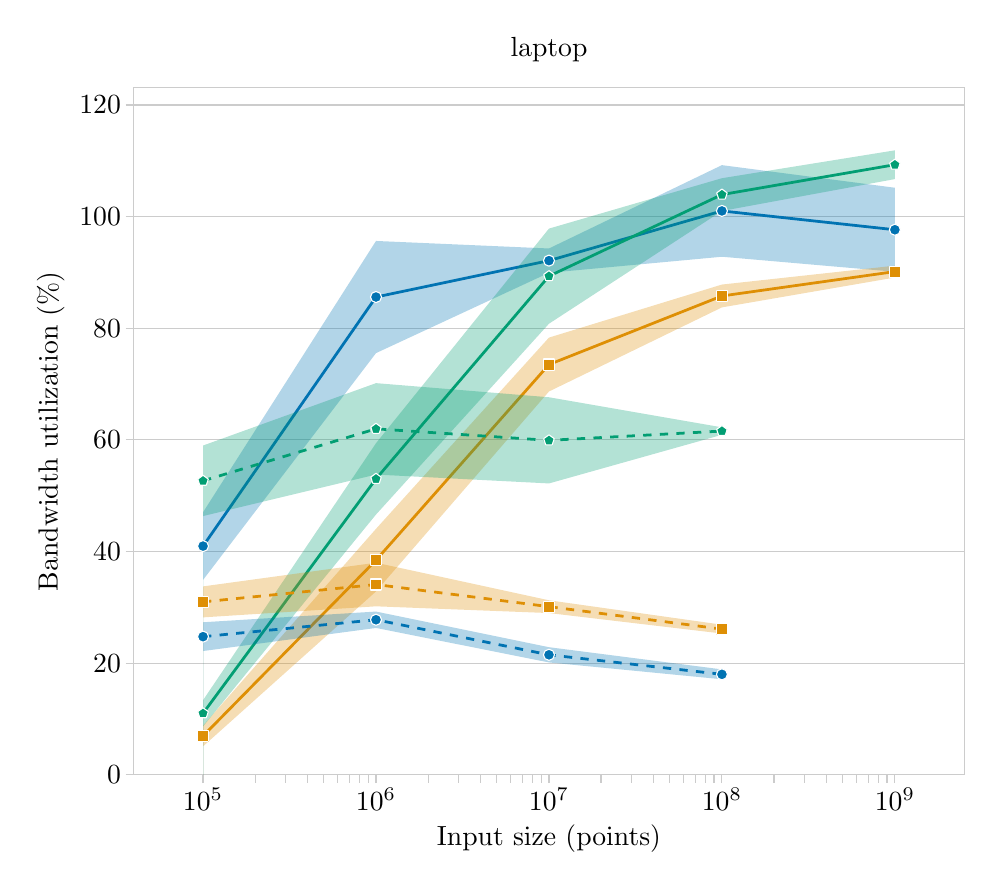
\begin{tikzpicture}
\begin{axis}[
  title={laptop},
  width=\epyfigurewidth,
  height={\epyheightratio*\epyfigurewidth},
  ymin=0,
  xlabel={Input size (points)},
  ylabel={Bandwidth utilization (\si{{\percent}})},
  xmode=log,
  scaled ticks=false,
  xtick={100000,1000000,10000000,100000000,1000000000},
  extra y ticks={\pgfkeysvalueof{/pgfplots/ymax}},
  extra y tick labels={\vphantom{Ag}},
  tick pos=left,
  tick align=outside,
  ymajorgrids,
  legend cell align=left,
  major tick length=0.3em,
  /pgf/number format/fixed,
  axis line style={color=black!20},
  y grid style={color=black!20,line width=0.4pt},
  tick style={color=black!20,line width=0.4pt},
  tick label style={inner sep=0.15em},
  ylabel style={outer sep=-0.25em},
  extra y tick style={grid=none,major tick length=0pt,yticklabel style={opacity=0,text opacity=0}},
  legend style={draw=black!20,draw opacity=1,fill opacity=0.9,text opacity=1,inner sep=0.2em},
  legend image code/.code={\path[#1] (0em,0pt) -- (1.4em,0pt) plot coordinates {(0.7em,0pt)};},
]
\addplot[draw=none,fill=colorblind0,fill opacity=0.3,forget plot] coordinates {
  (100000,47.04183047982237)
  (1000000,95.64175127891542)
  (10000000,94.29367321659366)
  (100000000,109.22229042230371)
  (1000000000,105.17550131553412)
  (1000000000,90.12170162549913)
  (100000000,92.81285714498604)
  (10000000,89.942359427179)
  (1000000,75.55213330197856)
  (100000,34.92193257802817)
} \closedcycle;
\addplot[color=colorblind0,line width=1pt,mark=*,mark size=2pt,mark options={draw=white,line width=-0.4pt,solid}] coordinates {
  (100000,40.98188152892527)
  (1000000,85.59694229044699)
  (10000000,92.11801632188633)
  (100000000,101.01757378364488)
  (1000000000,97.64860147051662)
};
\addplot[draw=none,fill=colorblind1,fill opacity=0.3,forget plot] coordinates {
  (100000,8.822462001496552)
  (1000000,44.07426678443832)
  (10000000,78.33188470866209)
  (100000000,87.83398264912728)
  (1000000000,91.21537629503305)
  (1000000000,89.09095021773314)
  (100000000,83.73998601590347)
  (10000000,68.67716041663071)
  (1000000,32.8585104180532)
  (100000,5.109072417410537)
} \closedcycle;
\addplot[color=colorblind1,line width=1pt,mark=square*,mark size=2pt,mark options={draw=white,line width=-0.4pt,solid}] coordinates {
  (100000,6.965767209453545)
  (1000000,38.46638860124576)
  (10000000,73.5045225626464)
  (100000000,85.78698433251537)
  (1000000000,90.1531632563831)
};
\addplot[draw=none,fill=colorblind2,fill opacity=0.3,forget plot] coordinates {
  (100000,13.38222771276498)
  (1000000,59.415892042977106)
  (10000000,97.85375114900083)
  (100000000,106.88003836339672)
  (1000000000,111.87485331757372)
  (1000000000,106.7264678763506)
  (100000000,101.01146848020753)
  (10000000,80.8191591708937)
  (1000000,46.63653834480742)
  (100000,8.682081043651003)
} \closedcycle;
\addplot[color=colorblind2,line width=1pt,mark=pentagon*,mark size=2pt,mark options={draw=white,line width=-0.4pt,solid}] coordinates {
  (100000,11.032154378207991)
  (1000000,53.02621519389226)
  (10000000,89.33645515994726)
  (100000000,103.94575342180212)
  (1000000000,109.30066059696216)
};
\addplot[draw=none,fill=colorblind0,fill opacity=0.3,forget plot] coordinates {
  (100000,27.339285196469486)
  (1000000,29.257600121326924)
  (10000000,22.873339494954617)
  (100000000,18.895870217699144)
  (100000000,17.127617431981836)
  (10000000,20.1425721126132)
  (1000000,26.3200425542896)
  (100000,22.185104413077052)
} \closedcycle;
\addplot[color=colorblind0,line width=1pt,dashed,mark=*,mark size=2pt,mark options={draw=white,line width=-0.4pt,solid}] coordinates {
  (100000,24.76219480477327)
  (1000000,27.788821337808262)
  (10000000,21.507955803783908)
  (100000000,18.01174382484049)
};
\addplot[draw=none,fill=colorblind1,fill opacity=0.3,forget plot] coordinates {
  (100000,33.76420780774549)
  (1000000,38.005848048854396)
  (10000000,31.27662325992016)
  (100000000,26.902793548396563)
  (100000000,25.32221703659626)
  (10000000,28.98822171920583)
  (1000000,30.19523905248834)
  (100000,28.213639803740264)
} \closedcycle;
\addplot[color=colorblind1,line width=1pt,dashed,mark=square*,mark size=2pt,mark options={draw=white,line width=-0.4pt,solid}] coordinates {
  (100000,30.98892380574288)
  (1000000,34.10054355067137)
  (10000000,30.132422489562995)
  (100000000,26.11250529249641)
};
\addplot[draw=none,fill=colorblind2,fill opacity=0.3,forget plot] coordinates {
  (100000,58.99491467840087)
  (1000000,70.17148609653687)
  (10000000,67.64231332117741)
  (100000000,62.25575750689544)
  (100000000,60.92128495371775)
  (10000000,52.20636928763799)
  (1000000,53.79876979967048)
  (100000,46.36357801906423)
} \closedcycle;
\addplot[color=colorblind2,line width=1pt,dashed,mark=pentagon*,mark size=2pt,mark options={draw=white,line width=-0.4pt,solid}] coordinates {
  (100000,52.67924634873255)
  (1000000,61.985127948103674)
  (10000000,59.924341304407704)
  (100000000,61.5885212303066)
};
\end{axis}%
\end{tikzpicture}%%
  \end{subfigure}%
  \caption{Bandwidth utilization over input sweep as a percentage of STREAM's
  bandwidth, fixed at the maximum number of available threads. The solid lines
  represent the VQhull implementation, the dashed lines represent the PBBS
  implementation.}%
\end{figure}

\begin{figure}
  \scriptsize
  \begin{subfigure}{.333\linewidth}
    \centering
    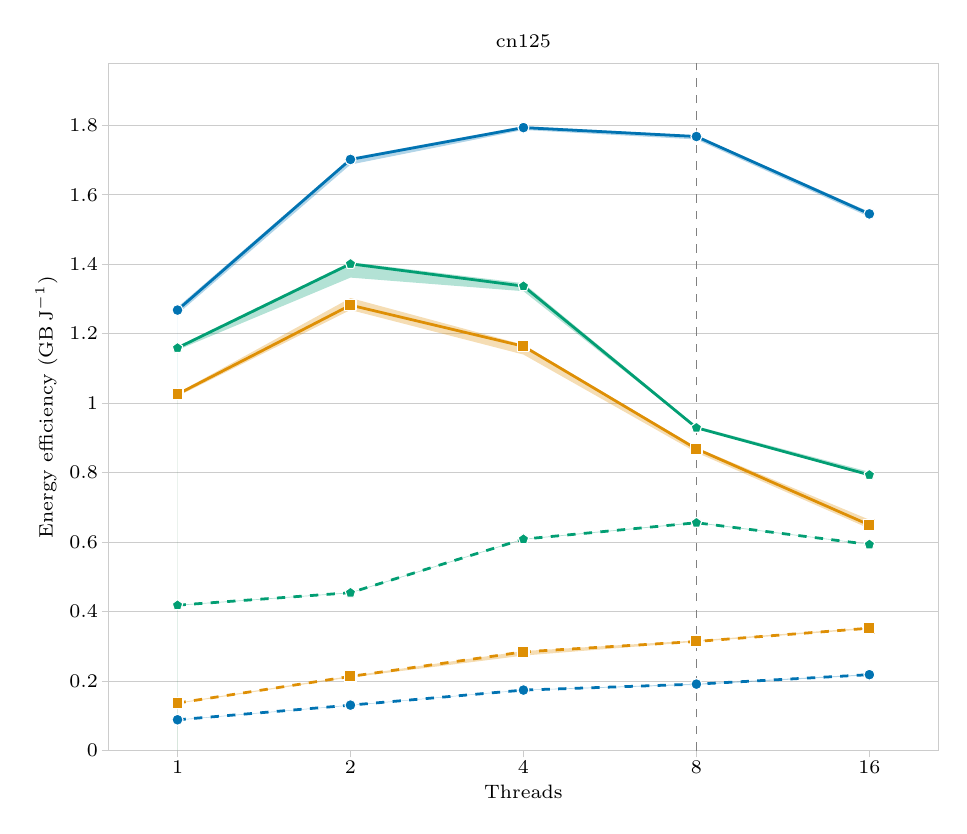
\begin{tikzpicture}
\scriptsize
\begin{axis}[
  title={cn125},
  width=\epyfigurewidth,
  height={\epyheightratio*\epyfigurewidth},
  ymin=0,
  xlabel={Threads},
  ylabel={Energy efficiency (\si{\giga\byte\per\joule})},
  xmode=log,
  scaled ticks=false,
  xtick={1,2,4,8,16},
  extra y ticks={\pgfkeysvalueof{/pgfplots/ymax}},
  xticklabels={1,2,4,8,16},
  extra y tick labels={\vphantom{Ag}},
  tick pos=left,
  tick align=outside,
  ymajorgrids,
  legend cell align=left,
  major tick length=0.3em,
  /pgf/number format/fixed,
  axis line style={color=black!20},
  y grid style={color=black!20,line width=0.4pt},
  title style={yshift=-1ex},
  tick style={color=black!20,line width=0.4pt},
  tick label style={inner sep=0.15em},
  ylabel style={outer sep=-0.25em},
  extra y tick style={grid=none,major tick length=0pt,yticklabel style={opacity=0,text opacity=0}},
  legend style={draw=black!20,draw opacity=1,fill opacity=0.9,text opacity=1,inner sep=0.2em},
  legend image code/.code={\path[#1] (0em,0pt) -- (1.4em,0pt) plot coordinates {(0.7em,0pt)};},
]
\addplot[draw=none,fill=colorblind0,fill opacity=0.3,forget plot] coordinates {
  (1,1.276329018558754)
  (2,1.7061680994574355)
  (4,1.7975224253337512)
  (8,1.7710066726891671)
  (16,1.5506948631146407)
  (16,1.5361635159664162)
  (8,1.7592530134368172)
  (4,1.786577158685364)
  (2,1.6868413649453255)
  (1,1.2563937554108533)
} \closedcycle;
\addplot[color=colorblind0,line width=1pt,mark=*,mark size=2pt,mark options={draw=white,line width=-0.4pt,solid}] coordinates {
  (1,1.2681008425626707)
  (2,1.7016412341749874)
  (4,1.79327485085601)
  (8,1.7676881609151711)
  (16,1.5449700166006946)
};
\addplot[draw=none,fill=colorblind1,fill opacity=0.3,forget plot] coordinates {
  (1,1.029491541646957)
  (2,1.302876546801578)
  (4,1.1684814568107387)
  (8,0.8723319885914709)
  (16,0.6647497669412863)
  (16,0.6390488706042714)
  (8,0.858195588856299)
  (4,1.1401191590918773)
  (2,1.2683985481082627)
  (1,1.0200781695568322)
} \closedcycle;
\addplot[color=colorblind1,line width=1pt,mark=square*,mark size=2pt,mark options={draw=white,line width=-0.4pt,solid}] coordinates {
  (1,1.0258425214619042)
  (2,1.282355169912956)
  (4,1.16404283974348)
  (8,0.8686314175636622)
  (16,0.6496852318233329)
};
\addplot[draw=none,fill=colorblind2,fill opacity=0.3,forget plot] coordinates {
  (1,1.1639332416143655)
  (2,1.4060036570663286)
  (4,1.3453800228383395)
  (8,0.933804619032839)
  (16,0.8024673541848344)
  (16,0.790321440413323)
  (8,0.928163584334095)
  (4,1.3224586565597338)
  (2,1.3615927415487719)
  (1,1.1530764036440095)
} \closedcycle;
\addplot[color=colorblind2,line width=1pt,mark=pentagon*,mark size=2pt,mark options={draw=white,line width=-0.4pt,solid}] coordinates {
  (1,1.1592327806996183)
  (2,1.4012054012524304)
  (4,1.337017076201755)
  (8,0.9294649212500365)
  (16,0.7939174042591903)
};
\addplot[draw=none,fill=colorblind0,fill opacity=0.3,forget plot] coordinates {
  (1,0.08923755554908293)
  (2,0.13138149754328332)
  (4,0.17505366496471275)
  (8,0.1927026135840852)
  (16,0.2200634032411107)
  (16,0.21724481162844797)
  (8,0.18945365456938726)
  (4,0.17384462554250396)
  (2,0.12991482780518568)
  (1,0.08772676830827511)
} \closedcycle;
\addplot[color=colorblind0,line width=1pt,dashed,mark=*,mark size=2pt,mark options={draw=white,line width=-0.4pt,solid}] coordinates {
  (1,0.08896579671787283)
  (2,0.13109437687449188)
  (4,0.17441296557698674)
  (8,0.19157226328396026)
  (16,0.21880118545775745)
};
\addplot[draw=none,fill=colorblind1,fill opacity=0.3,forget plot] coordinates {
  (1,0.13801683584089305)
  (2,0.21497782141674943)
  (4,0.2868433459055822)
  (8,0.3173214350701123)
  (16,0.3544855424177959)
  (16,0.3502319322911483)
  (8,0.31338376258853773)
  (4,0.2736815132659659)
  (2,0.21096606923797473)
  (1,0.13552126215396187)
} \closedcycle;
\addplot[color=colorblind1,line width=1pt,dashed,mark=square*,mark size=2pt,mark options={draw=white,line width=-0.4pt,solid}] coordinates {
  (1,0.13714615126743213)
  (2,0.21371976129649864)
  (4,0.2844409693098223)
  (8,0.314316541253162)
  (16,0.3525588123344852)
};
\addplot[draw=none,fill=colorblind2,fill opacity=0.3,forget plot] coordinates {
  (1,0.41957488321453196)
  (2,0.4553740710610309)
  (4,0.6096557800442406)
  (8,0.6573442200223013)
  (16,0.5945267445271327)
  (16,0.5930528347612725)
  (8,0.6549485272625835)
  (4,0.6076646010989555)
  (2,0.4534286643066389)
  (1,0.41763522641841494)
} \closedcycle;
\addplot[color=colorblind2,line width=1pt,dashed,mark=pentagon*,mark size=2pt,mark options={draw=white,line width=-0.4pt,solid}] coordinates {
  (1,0.4188209605265828)
  (2,0.45476689380305635)
  (4,0.6089259877696434)
  (8,0.6560617535285747)
  (16,0.593543928071147)
};
\draw[draw=gray,dashed] (axis cs:8,0) -- (axis cs:8,5);
\end{axis}%
\end{tikzpicture}%%
  \end{subfigure}%
  \begin{subfigure}{.333\linewidth}
    \centering
    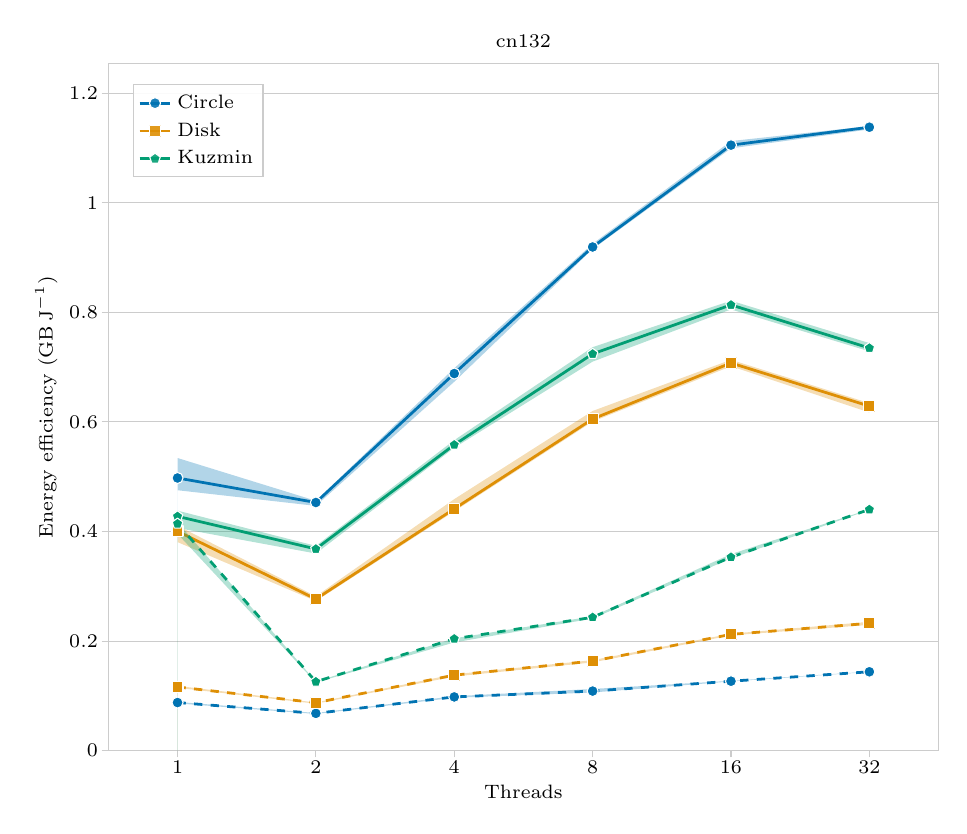
\begin{tikzpicture}
\scriptsize
\begin{axis}[
  title={cn132},
  width=\epyfigurewidth,
  height={\epyheightratio*\epyfigurewidth},
  ymin=0,
  xlabel={Threads},
  ylabel={Energy efficiency (\si{\giga\byte\per\joule})},
  xmode=log,
  scaled ticks=false,
  xtick={1,2,4,8,16,32},
  extra y ticks={\pgfkeysvalueof{/pgfplots/ymax}},
  xticklabels={1,2,4,8,16,32},
  extra y tick labels={\vphantom{Ag}},
  tick pos=left,
  tick align=outside,
  ymajorgrids,
  legend pos=north west,
  legend cell align=left,
  major tick length=0.3em,
  /pgf/number format/fixed,
  axis line style={color=black!20},
  y grid style={color=black!20,line width=0.4pt},
  title style={yshift=-1ex},
  tick style={color=black!20,line width=0.4pt},
  tick label style={inner sep=0.15em},
  ylabel style={outer sep=-0.25em},
  extra y tick style={grid=none,major tick length=0pt,yticklabel style={opacity=0,text opacity=0}},
  legend style={draw=black!20,draw opacity=1,fill opacity=0.9,text opacity=1,inner sep=0.2em},
  legend image code/.code={\path[#1] (0em,0pt) -- (1.4em,0pt) plot coordinates {(0.7em,0pt)};},
]
\addplot[draw=none,fill=colorblind0,fill opacity=0.3,forget plot] coordinates {
  (1,0.5341751098692948)
  (2,0.45611212915098437)
  (4,0.6980792303848139)
  (8,0.9251386853102344)
  (16,1.1126685776854106)
  (32,1.139905666198228)
  (32,1.13393577626826)
  (16,1.099359654959989)
  (8,0.9155290526475925)
  (4,0.6733023339842208)
  (2,0.44678783617284806)
  (1,0.47538130632001235)
} \closedcycle;
\addplot[color=colorblind0,line width=1pt,mark=*,mark size=2pt,mark options={draw=white,line width=-0.4pt,solid}] coordinates {
  (1,0.49773559047967275)
  (2,0.45297502999165645)
  (4,0.6883350798863268)
  (8,0.9193481485132233)
  (16,1.1052148170571927)
  (32,1.1379458544013654)
};
\addlegendentry{Circle}
\addplot[draw=none,fill=colorblind1,fill opacity=0.3,forget plot] coordinates {
  (1,0.4107368304619322)
  (2,0.28177655571004384)
  (4,0.4591918365475454)
  (8,0.6200242955029182)
  (16,0.7134542771809305)
  (32,0.6342782156803833)
  (32,0.6171890579415056)
  (16,0.7017437191509854)
  (8,0.6006631835392204)
  (4,0.4369438120134791)
  (2,0.27300905245024293)
  (1,0.3806806020316274)
} \closedcycle;
\addplot[color=colorblind1,line width=1pt,mark=square*,mark size=2pt,mark options={draw=white,line width=-0.4pt,solid}] coordinates {
  (1,0.400424637478739)
  (2,0.2767065293393037)
  (4,0.4414385423767131)
  (8,0.6054287016920121)
  (16,0.707630080764192)
  (32,0.6288540780391209)
};
\addlegendentry{Disk}
\addplot[draw=none,fill=colorblind2,fill opacity=0.3,forget plot] coordinates {
  (1,0.4381460221212044)
  (2,0.3738409435733082)
  (4,0.5667310028286451)
  (8,0.7364961955894328)
  (16,0.8213268911368832)
  (32,0.7439617866353844)
  (32,0.7288338619155807)
  (16,0.8053690697518371)
  (8,0.7100877937868202)
  (4,0.5528564952000804)
  (2,0.3598772113148826)
  (1,0.4064754641561911)
} \closedcycle;
\addplot[color=colorblind2,line width=1pt,mark=pentagon*,mark size=2pt,mark options={draw=white,line width=-0.4pt,solid}] coordinates {
  (1,0.427673210052388)
  (2,0.3682012006653028)
  (4,0.558354181987128)
  (8,0.7242391593065922)
  (16,0.8136509683193051)
  (32,0.7349387753016923)
};
\addlegendentry{Kuzmin}
\addplot[draw=none,fill=colorblind0,fill opacity=0.3,forget plot] coordinates {
  (1,0.08905564709662021)
  (2,0.06881021338242668)
  (4,0.09944659451536629)
  (8,0.11269189406497862)
  (16,0.12753331201582724)
  (32,0.14438037427092523)
  (32,0.14363688294556035)
  (16,0.1263699662284494)
  (8,0.10618128836879621)
  (4,0.0965603728426967)
  (2,0.06705358513915663)
  (1,0.08629101982746747)
} \closedcycle;
\addplot[color=colorblind0,line width=1pt,dashed,mark=*,mark size=2pt,mark options={draw=white,line width=-0.4pt,solid}] coordinates {
  (1,0.08785172543399661)
  (2,0.06812385968871532)
  (4,0.09811489582801444)
  (8,0.10878911769207911)
  (16,0.12683336088474256)
  (32,0.14400817623062317)
};
\addplot[draw=none,fill=colorblind1,fill opacity=0.3,forget plot] coordinates {
  (1,0.11823170515286868)
  (2,0.08793865636289154)
  (4,0.1394876299393191)
  (8,0.1652949925280773)
  (16,0.21352099075315123)
  (32,0.23524968717592973)
  (32,0.22964170520835142)
  (16,0.21042179660482177)
  (8,0.16110684634451414)
  (4,0.1353138803574847)
  (2,0.08575777177949334)
  (1,0.11472598597051342)
} \closedcycle;
\addplot[color=colorblind1,line width=1pt,dashed,mark=square*,mark size=2pt,mark options={draw=white,line width=-0.4pt,solid}] coordinates {
  (1,0.11626604615571062)
  (2,0.0875675321519798)
  (4,0.13790137384696755)
  (8,0.16356386897494213)
  (16,0.21228061125033681)
  (32,0.2324421570233688)
};
\addplot[draw=none,fill=colorblind2,fill opacity=0.3,forget plot] coordinates {
  (1,0.41689206363133513)
  (2,0.12611870002792117)
  (4,0.2050934324768768)
  (8,0.24518980596567327)
  (16,0.35880884782586653)
  (32,0.44059423076923826)
  (32,0.43936479348016294)
  (16,0.3509773118818429)
  (8,0.24116433126056983)
  (4,0.19758058479731905)
  (2,0.12437016806141092)
  (1,0.3957735066959424)
} \closedcycle;
\addplot[color=colorblind2,line width=1pt,dashed,mark=pentagon*,mark size=2pt,mark options={draw=white,line width=-0.4pt,solid}] coordinates {
  (1,0.41438919870793556)
  (2,0.12591215229961195)
  (4,0.20425742004325403)
  (8,0.24344498976300732)
  (16,0.3532736362057084)
  (32,0.44025785884152474)
};
\end{axis}%
\end{tikzpicture}%%
  \end{subfigure}%
  \begin{subfigure}{.333\linewidth}
    \centering
    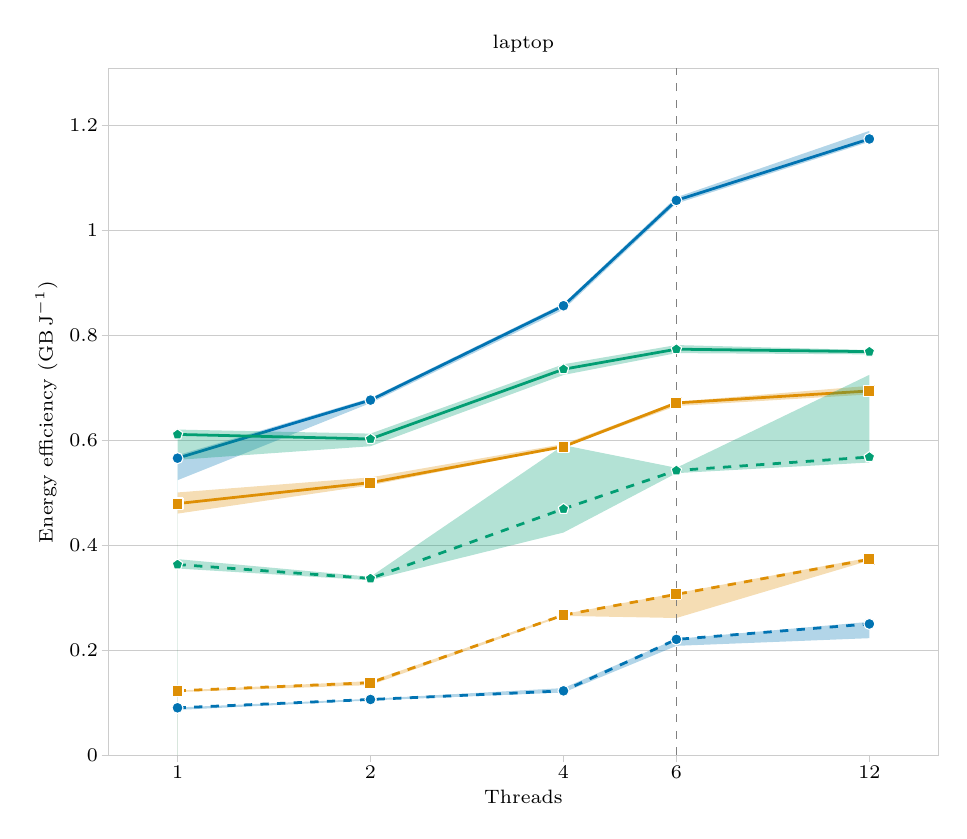
\begin{tikzpicture}
\scriptsize
\begin{axis}[
  title={laptop},
  width=\epyfigurewidth,
  height={\epyheightratio*\epyfigurewidth},
  ymin=0,
  xlabel={Threads},
  ylabel={Energy efficiency (\si{\giga\byte\per\joule})},
  xmode=log,
  scaled ticks=false,
  xtick={1,2,4,6,12},
  extra y ticks={\pgfkeysvalueof{/pgfplots/ymax}},
  xticklabels={1,2,4,6,12},
  extra y tick labels={\vphantom{Ag}},
  tick pos=left,
  tick align=outside,
  ymajorgrids,
  legend cell align=left,
  major tick length=0.3em,
  /pgf/number format/fixed,
  axis line style={color=black!20},
  y grid style={color=black!20,line width=0.4pt},
  title style={yshift=-1ex},
  tick style={color=black!20,line width=0.4pt},
  tick label style={inner sep=0.15em},
  ylabel style={outer sep=-0.25em},
  extra y tick style={grid=none,major tick length=0pt,yticklabel style={opacity=0,text opacity=0}},
  legend style={draw=black!20,draw opacity=1,fill opacity=0.9,text opacity=1,inner sep=0.2em},
  legend image code/.code={\path[#1] (0em,0pt) -- (1.4em,0pt) plot coordinates {(0.7em,0pt)};},
]
\addplot[draw=none,fill=colorblind0,fill opacity=0.3,forget plot] coordinates {
  (1,0.5717163643820896)
  (2,0.6805099044194726)
  (4,0.8605823325419075)
  (6,1.06311136471031)
  (12,1.1896296338898185)
  (12,1.1688475851723432)
  (6,1.0512075249732935)
  (4,0.8493250402904857)
  (2,0.671131180155984)
  (1,0.5242038837631408)
} \closedcycle;
\addplot[color=colorblind0,line width=1pt,mark=*,mark size=2pt,mark options={draw=white,line width=-0.4pt,solid}] coordinates {
  (1,0.5662095114262667)
  (2,0.6768270357232603)
  (4,0.856537161389185)
  (6,1.05726247654246)
  (12,1.1742473987615547)
};
\addplot[draw=none,fill=colorblind1,fill opacity=0.3,forget plot] coordinates {
  (1,0.5008907735422286)
  (2,0.5295482082327164)
  (4,0.593058990756938)
  (6,0.6735591013189881)
  (12,0.704073692830588)
  (12,0.6875988554661085)
  (6,0.6655052494357664)
  (4,0.5868324266840599)
  (2,0.5145307768353881)
  (1,0.46055787402808557)
} \closedcycle;
\addplot[color=colorblind1,line width=1pt,mark=square*,mark size=2pt,mark options={draw=white,line width=-0.4pt,solid}] coordinates {
  (1,0.47969793263455984)
  (2,0.5196181553552236)
  (4,0.5881850401035922)
  (6,0.671453928129752)
  (12,0.6942928198371288)
};
\addplot[draw=none,fill=colorblind2,fill opacity=0.3,forget plot] coordinates {
  (1,0.6206624485733276)
  (2,0.6129544513986821)
  (4,0.745073245943608)
  (6,0.7816745362859154)
  (12,0.772107539707809)
  (12,0.7639305157294266)
  (6,0.7663110247514389)
  (4,0.7247094027667014)
  (2,0.5889558463636302)
  (1,0.5629331479743671)
} \closedcycle;
\addplot[color=colorblind2,line width=1pt,mark=pentagon*,mark size=2pt,mark options={draw=white,line width=-0.4pt,solid}] coordinates {
  (1,0.6114331475715686)
  (2,0.6028711551309407)
  (4,0.7356044336876821)
  (6,0.7737970100501226)
  (12,0.7691143047238309)
};
\addplot[draw=none,fill=colorblind0,fill opacity=0.3,forget plot] coordinates {
  (1,0.09132759015601728)
  (2,0.10788672450080579)
  (4,0.12827448267849556)
  (6,0.22202037591379017)
  (12,0.25446356440606593)
  (12,0.22332729658092174)
  (6,0.20872093502145014)
  (4,0.11979197737522572)
  (2,0.10476257021599823)
  (1,0.0866355247069261)
} \closedcycle;
\addplot[color=colorblind0,line width=1pt,dashed,mark=*,mark size=2pt,mark options={draw=white,line width=-0.4pt,solid}] coordinates {
  (1,0.09067852691091356)
  (2,0.10657145982862283)
  (4,0.12296904726783212)
  (6,0.2210202998848015)
  (12,0.2504687377786716)
};
\addplot[draw=none,fill=colorblind1,fill opacity=0.3,forget plot] coordinates {
  (1,0.123562979555273)
  (2,0.14162602304849178)
  (4,0.2691826766447718)
  (6,0.30915650298937714)
  (12,0.37659736574525526)
  (12,0.3712202555014886)
  (6,0.2617819131942864)
  (4,0.2657497758781527)
  (2,0.13396410640267134)
  (1,0.12068541708976796)
} \closedcycle;
\addplot[color=colorblind1,line width=1pt,dashed,mark=square*,mark size=2pt,mark options={draw=white,line width=-0.4pt,solid}] coordinates {
  (1,0.1231343133164784)
  (2,0.13847792805015302)
  (4,0.2673820058999449)
  (6,0.306879331280997)
  (12,0.37350867749976596)
};
\addplot[draw=none,fill=colorblind2,fill opacity=0.3,forget plot] coordinates {
  (1,0.37392496383101614)
  (2,0.340342328729894)
  (4,0.5909224425826957)
  (6,0.5477945211127635)
  (12,0.7249431962813514)
  (12,0.5579722944087722)
  (6,0.5376743121342343)
  (4,0.4245911194420115)
  (2,0.3336674214866671)
  (1,0.3560275859753978)
} \closedcycle;
\addplot[color=colorblind2,line width=1pt,dashed,mark=pentagon*,mark size=2pt,mark options={draw=white,line width=-0.4pt,solid}] coordinates {
  (1,0.3637049258292585)
  (2,0.3371056113351337)
  (4,0.4696557611767319)
  (6,0.5427328178005153)
  (12,0.5683863777896059)
};
\draw[draw=gray,dashed] (axis cs:6,0) -- (axis cs:6,5);
\end{axis}%
\end{tikzpicture}%%
  \end{subfigure}%
  \caption{Energy efficiency for $10^8$ points. The solid lines represent the
  VQhull implementation, the dashed lines represent the PBBS implementation.}%
\end{figure}

\begin{figure}
  \scriptsize
  \begin{subfigure}{.333\linewidth}
    \centering
    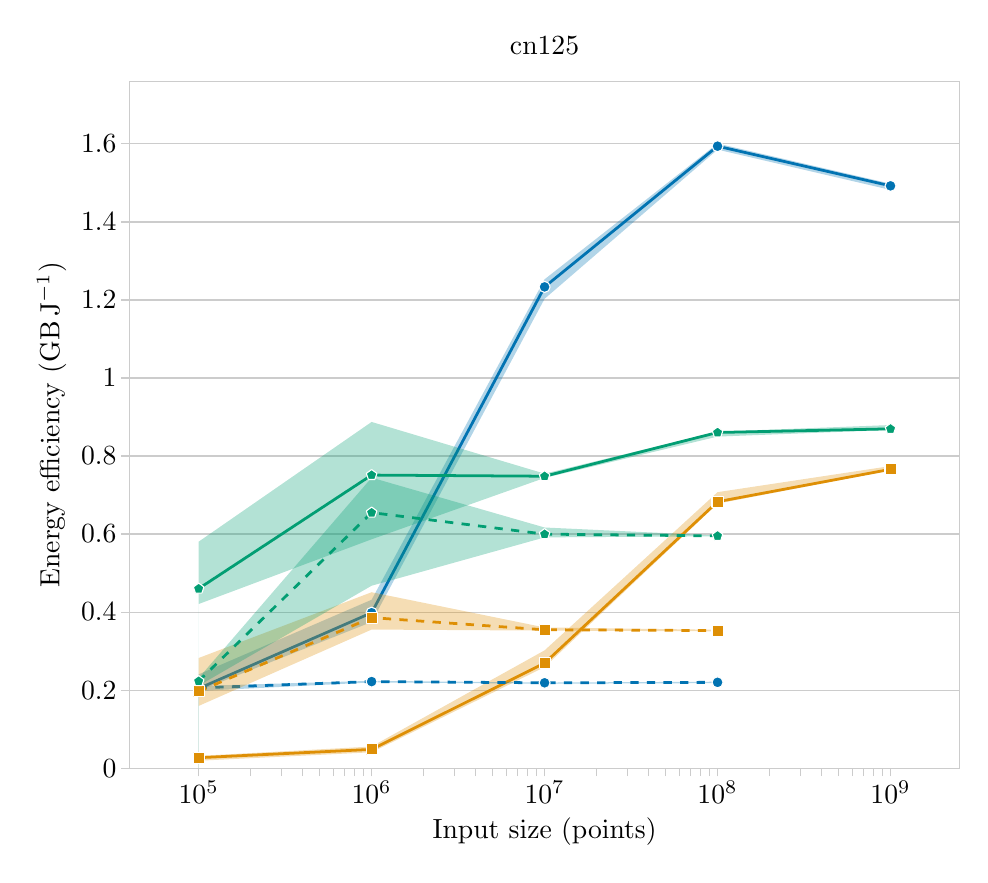
\begin{tikzpicture}
\begin{axis}[
  title={cn125},
  width=\epyfigurewidth,
  height={\epyheightratio*\epyfigurewidth},
  ymin=0,
  xlabel={Input size (points)},
  ylabel={Energy efficiency (\si{\giga\byte\per\joule})},
  xmode=log,
  scaled ticks=false,
  xtick={100000,1000000,10000000,100000000,1000000000},
  extra y ticks={\pgfkeysvalueof{/pgfplots/ymax}},
  extra y tick labels={\vphantom{Ag}},
  tick pos=left,
  tick align=outside,
  ymajorgrids,
  legend cell align=left,
  major tick length=0.3em,
  /pgf/number format/fixed,
  axis line style={color=black!20},
  y grid style={color=black!20,line width=0.4pt},
  tick style={color=black!20,line width=0.4pt},
  tick label style={inner sep=0.15em},
  ylabel style={outer sep=-0.25em},
  extra y tick style={grid=none,major tick length=0pt,yticklabel style={opacity=0,text opacity=0}},
  legend style={draw=black!20,draw opacity=1,fill opacity=0.9,text opacity=1,inner sep=0.2em},
  legend image code/.code={\path[#1] (0em,0pt) -- (1.4em,0pt) plot coordinates {(0.7em,0pt)};},
]
\addplot[draw=none,fill=colorblind0,fill opacity=0.3,forget plot] coordinates {
  (100000,0.24045920275892496)
  (1000000,0.4316399241441271)
  (10000000,1.2530283658765144)
  (100000000,1.600926109039876)
  (1000000000,1.4980920058144354)
  (1000000000,1.4820980599037596)
  (100000000,1.5854212457313515)
  (10000000,1.203020674813085)
  (1000000,0.37459992805836806)
  (100000,0.19825659408636018)
} \closedcycle;
\addplot[color=colorblind0,line width=1pt,mark=*,mark size=2pt,mark options={draw=white,line width=-0.4pt,solid}] coordinates {
  (100000,0.20403336943382086)
  (1000000,0.3982998380907624)
  (10000000,1.2335309959660279)
  (100000000,1.5942087514125918)
  (1000000000,1.492516013651433)
};
\addplot[draw=none,fill=colorblind1,fill opacity=0.3,forget plot] coordinates {
  (100000,0.0312871812580624)
  (1000000,0.055369916532212606)
  (10000000,0.3018714808470445)
  (100000000,0.7073855935836924)
  (1000000000,0.7743047372962913)
  (1000000000,0.7633867133110062)
  (100000000,0.6779950786043484)
  (10000000,0.25897366711997555)
  (1000000,0.04058441548847775)
  (100000,0.018958295558174836)
} \closedcycle;
\addplot[color=colorblind1,line width=1pt,mark=square*,mark size=2pt,mark options={draw=white,line width=-0.4pt,solid}] coordinates {
  (100000,0.026695774838892225)
  (1000000,0.04801238683056607)
  (10000000,0.2691712112835576)
  (100000000,0.6829106668998947)
  (1000000000,0.7659420912993248)
};
\addplot[draw=none,fill=colorblind2,fill opacity=0.3,forget plot] coordinates {
  (100000,0.5804289360508055)
  (1000000,0.8873509611215407)
  (10000000,0.754778457178235)
  (100000000,0.862351748449703)
  (1000000000,0.8793990845135409)
  (1000000000,0.8669139550985309)
  (100000000,0.8498255253947421)
  (10000000,0.7439056211067069)
  (1000000,0.586587740778629)
  (100000,0.4206811362901617)
} \closedcycle;
\addplot[color=colorblind2,line width=1pt,mark=pentagon*,mark size=2pt,mark options={draw=white,line width=-0.4pt,solid}] coordinates {
  (100000,0.46007335822157175)
  (1000000,0.7511692775691236)
  (10000000,0.748233219280997)
  (100000000,0.860371538501469)
  (1000000000,0.869623499301913)
};
\addplot[draw=none,fill=colorblind0,fill opacity=0.3,forget plot] coordinates {
  (100000,0.21051266766330412)
  (1000000,0.2237332906381709)
  (10000000,0.21931039074367356)
  (100000000,0.22150875290719207)
  (100000000,0.21782116881898655)
  (10000000,0.2163864428032086)
  (1000000,0.2196715041762381)
  (100000,0.19775368439666394)
} \closedcycle;
\addplot[color=colorblind0,line width=1pt,dashed,mark=*,mark size=2pt,mark options={draw=white,line width=-0.4pt,solid}] coordinates {
  (100000,0.2056765199446622)
  (1000000,0.22183749246808546)
  (10000000,0.21869938081416615)
  (100000000,0.21991350880576038)
};
\addplot[draw=none,fill=colorblind1,fill opacity=0.3,forget plot] coordinates {
  (100000,0.2822773328510214)
  (1000000,0.4508825093186325)
  (10000000,0.36065433235631034)
  (100000000,0.3545286509679521)
  (100000000,0.35063399879458873)
  (10000000,0.3526080308297926)
  (1000000,0.35516824918931955)
  (100000,0.15941784055596192)
} \closedcycle;
\addplot[color=colorblind1,line width=1pt,dashed,mark=square*,mark size=2pt,mark options={draw=white,line width=-0.4pt,solid}] coordinates {
  (100000,0.19669981422795327)
  (1000000,0.385740603344799)
  (10000000,0.3545890690488093)
  (100000000,0.3526559044325205)
};
\addplot[draw=none,fill=colorblind2,fill opacity=0.3,forget plot] coordinates {
  (100000,0.23089908083490668)
  (1000000,0.7445076213126945)
  (10000000,0.616782762297869)
  (100000000,0.5961666078001191)
  (100000000,0.5942054313621223)
  (10000000,0.5914659986080315)
  (1000000,0.4675657260187648)
  (100000,0.211332535913564)
} \closedcycle;
\addplot[color=colorblind2,line width=1pt,dashed,mark=pentagon*,mark size=2pt,mark options={draw=white,line width=-0.4pt,solid}] coordinates {
  (100000,0.2229428455614106)
  (1000000,0.6549622543667207)
  (10000000,0.5997440553511298)
  (100000000,0.5952805520149631)
};
\end{axis}
\end{tikzpicture}%
  \end{subfigure}%
  \begin{subfigure}{.333\linewidth}
    \centering
    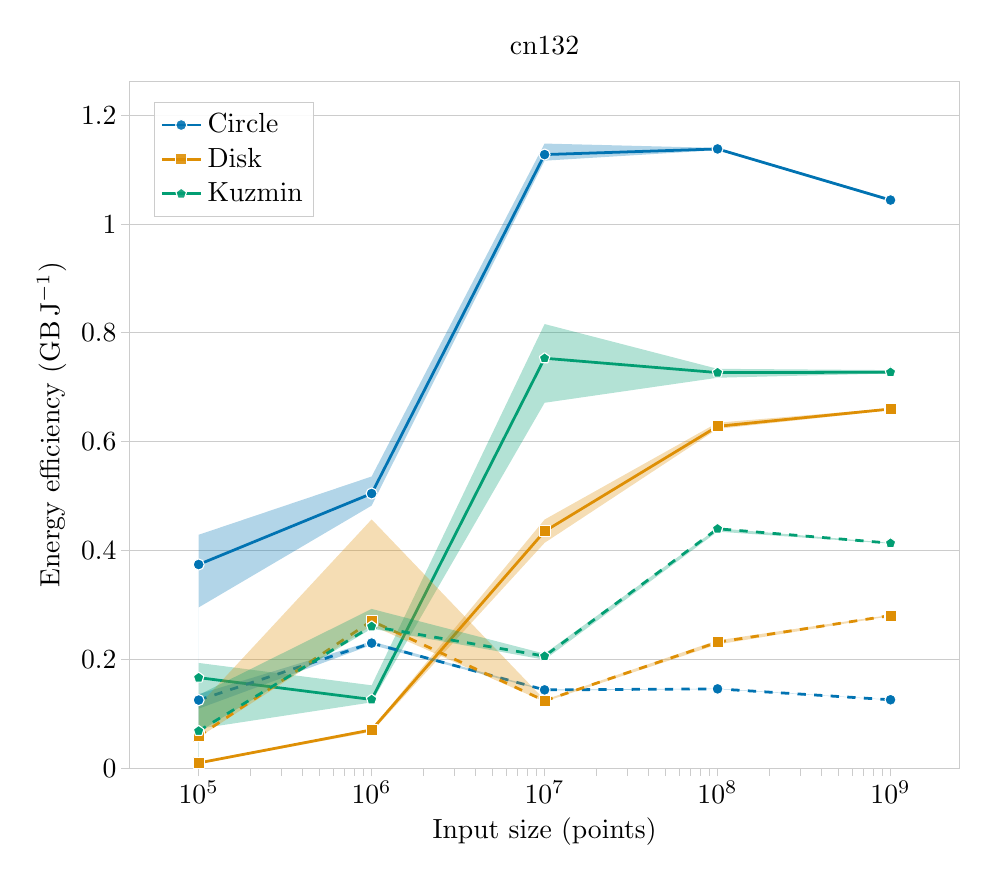
\begin{tikzpicture}
\begin{axis}[
  title={cn132},
  width=\epyfigurewidth,
  height={\epyheightratio*\epyfigurewidth},
  ymin=0,
  xlabel={Input size (points)},
  ylabel={Energy efficiency (\si{\giga\byte\per\joule})},
  xmode=log,
  scaled ticks=false,
  xtick={100000,1000000,10000000,100000000,1000000000},
  extra y ticks={\pgfkeysvalueof{/pgfplots/ymax}},
  extra y tick labels={\vphantom{Ag}},
  tick pos=left,
  tick align=outside,
  ymajorgrids,
  legend pos=north west,
  legend cell align=left,
  major tick length=0.3em,
  /pgf/number format/fixed,
  axis line style={color=black!20},
  y grid style={color=black!20,line width=0.4pt},
  tick style={color=black!20,line width=0.4pt},
  tick label style={inner sep=0.15em},
  ylabel style={outer sep=-0.25em},
  extra y tick style={grid=none,major tick length=0pt,yticklabel style={opacity=0,text opacity=0}},
  legend style={draw=black!20,draw opacity=1,fill opacity=0.9,text opacity=1,inner sep=0.2em},
  legend image code/.code={\path[#1] (0em,0pt) -- (1.4em,0pt) plot coordinates {(0.7em,0pt)};},
]
\addplot[draw=none,fill=colorblind0,fill opacity=0.3,forget plot] coordinates {
  (100000,0.4289210533288935)
  (1000000,0.5360284637487729)
  (10000000,1.1479963240656623)
  (100000000,1.140003996735933)
  (1000000000,1.0467408165046397)
  (1000000000,1.0418259500960432)
  (100000000,1.135931557991624)
  (10000000,1.1165247582768425)
  (1000000,0.4825243426421445)
  (100000,0.29540171324988235)
} \closedcycle;
\addplot[color=colorblind0,line width=1pt,mark=*,mark size=2pt,mark options={draw=white,line width=-0.4pt,solid}] coordinates {
  (100000,0.3742686195270306)
  (1000000,0.5047175318137671)
  (10000000,1.1277324604145855)
  (100000000,1.1381340514363574)
  (1000000000,1.0441355952258458)
};
\addlegendentry{Circle}
\addplot[draw=none,fill=colorblind1,fill opacity=0.3,forget plot] coordinates {
  (100000,0.010398781104296935)
  (1000000,0.07249451960735608)
  (10000000,0.45688429088580973)
  (100000000,0.6349532759921765)
  (1000000000,0.6614935967455344)
  (1000000000,0.6579507905299098)
  (100000000,0.6235336313053501)
  (10000000,0.4141067932775463)
  (1000000,0.06670103835315991)
  (100000,0.007876550473469152)
} \closedcycle;
\addplot[color=colorblind1,line width=1pt,mark=square*,mark size=2pt,mark options={draw=white,line width=-0.4pt,solid}] coordinates {
  (100000,0.009514411944786395)
  (1000000,0.07033569521027366)
  (10000000,0.4352485672938665)
  (100000000,0.6282317192121976)
  (1000000000,0.6600971281874425)
};
\addlegendentry{Disk}
\addplot[draw=none,fill=colorblind2,fill opacity=0.3,forget plot] coordinates {
  (100000,0.19334357732221705)
  (1000000,0.15220211708449893)
  (10000000,0.8162371304825126)
  (100000000,0.73393563216664)
  (1000000000,0.7315631018191228)
  (1000000000,0.7254811394266752)
  (100000000,0.7175723738903267)
  (10000000,0.6715695596286952)
  (1000000,0.12086510766273015)
  (100000,0.0723377856747409)
} \closedcycle;
\addplot[color=colorblind2,line width=1pt,mark=pentagon*,mark size=2pt,mark options={draw=white,line width=-0.4pt,solid}] coordinates {
  (100000,0.16630824131179645)
  (1000000,0.12613793273500148)
  (10000000,0.7534031255546391)
  (100000000,0.7270438492324145)
  (1000000000,0.7276753248715526)
};
\addlegendentry{Kuzmin}
\addplot[draw=none,fill=colorblind0,fill opacity=0.3,forget plot] coordinates {
  (100000,0.13587880323011114)
  (1000000,0.23309611483823509)
  (10000000,0.1444506731367624)
  (100000000,0.1460888558838439)
  (1000000000,0.1257292217865186)
  (1000000000,0.12534515049251801)
  (100000000,0.14517982564435508)
  (10000000,0.14259968217336666)
  (1000000,0.22641411100747333)
  (100000,0.10927485647531092)
} \closedcycle;
\addplot[color=colorblind0,line width=1pt,dashed,mark=*,mark size=2pt,mark options={draw=white,line width=-0.4pt,solid}] coordinates {
  (100000,0.12502303193419878)
  (1000000,0.2297805700708342)
  (10000000,0.14381689495881073)
  (100000000,0.1456576404550829)
  (1000000000,0.12562258400540582)
};
\addplot[draw=none,fill=colorblind1,fill opacity=0.3,forget plot] coordinates {
  (100000,0.11485661702957019)
  (1000000,0.4571678585808892)
  (10000000,0.1255400029712652)
  (100000000,0.2349136783688483)
  (1000000000,0.28165147191299006)
  (1000000000,0.27940092004750955)
  (100000000,0.22723571592433434)
  (10000000,0.12200989677715035)
  (1000000,0.2621899784161491)
  (100000,0.056410863781779993)
} \closedcycle;
\addplot[color=colorblind1,line width=1pt,dashed,mark=square*,mark size=2pt,mark options={draw=white,line width=-0.4pt,solid}] coordinates {
  (100000,0.058640089272424305)
  (1000000,0.2705773278447242)
  (10000000,0.12387430324469698)
  (100000000,0.23143240432597706)
  (1000000000,0.2804130827737666)
};
\addplot[draw=none,fill=colorblind2,fill opacity=0.3,forget plot] coordinates {
  (100000,0.13449766980996644)
  (1000000,0.2926262180511637)
  (10000000,0.21031620052245986)
  (100000000,0.44094669526626035)
  (1000000000,0.4139576730349153)
  (1000000000,0.41269519457411696)
  (100000000,0.4347140832560845)
  (10000000,0.19929078457130575)
  (1000000,0.25641953658681327)
  (100000,0.06674774722812077)
} \closedcycle;
\addplot[color=colorblind2,line width=1pt,dashed,mark=pentagon*,mark size=2pt,mark options={draw=white,line width=-0.4pt,solid}] coordinates {
  (100000,0.0683606646520986)
  (1000000,0.2606086489393795)
  (10000000,0.20587162949416038)
  (100000000,0.4399599237480978)
  (1000000000,0.4135039675798936)
};
\end{axis}%
\end{tikzpicture}%%
  \end{subfigure}%
  \begin{subfigure}{.333\linewidth}
    \centering
    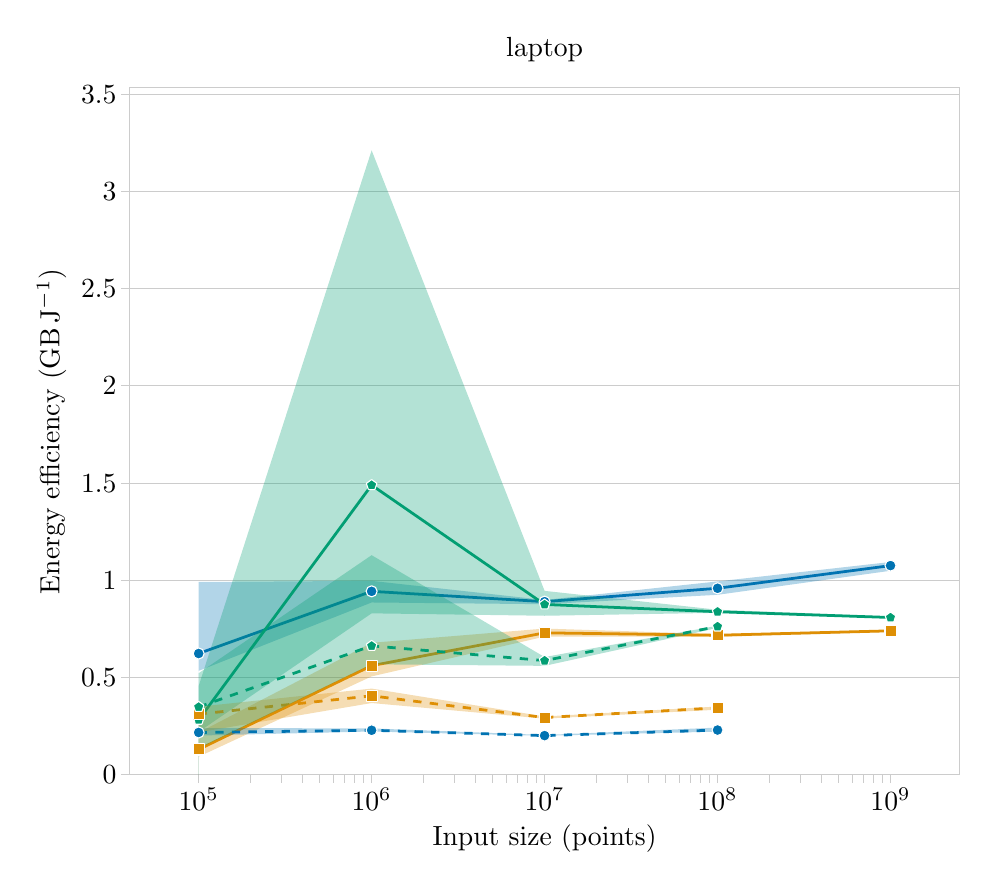
\begin{tikzpicture}
\begin{axis}[
  title={laptop},
  width=\epyfigurewidth,
  height={\epyheightratio*\epyfigurewidth},
  ymin=0,
  xlabel={Input size (points)},
  ylabel={Energy efficiency (\si{\giga\byte\per\joule})},
  xmode=log,
  scaled ticks=false,
  xtick={100000,1000000,10000000,100000000,1000000000},
  extra y ticks={\pgfkeysvalueof{/pgfplots/ymax}},
  extra y tick labels={\vphantom{Ag}},
  tick pos=left,
  tick align=outside,
  ymajorgrids,
  legend cell align=left,
  major tick length=0.3em,
  /pgf/number format/fixed,
  axis line style={color=black!20},
  y grid style={color=black!20,line width=0.4pt},
  tick style={color=black!20,line width=0.4pt},
  tick label style={inner sep=0.15em},
  ylabel style={outer sep=-0.25em},
  extra y tick style={grid=none,major tick length=0pt,yticklabel style={opacity=0,text opacity=0}},
  legend style={draw=black!20,draw opacity=1,fill opacity=0.9,text opacity=1,inner sep=0.2em},
  legend image code/.code={\path[#1] (0em,0pt) -- (1.4em,0pt) plot coordinates {(0.7em,0pt)};},
]
\addplot[draw=none,fill=colorblind0,fill opacity=0.3,forget plot] coordinates {
  (100000,0.9918925909816805)
  (1000000,0.9976278456319677)
  (10000000,0.8992728877325525)
  (100000000,0.9947906805788964)
  (1000000000,1.0947006341275254)
  (1000000000,1.0496076610307767)
  (100000000,0.9258647031891991)
  (10000000,0.8776939508245847)
  (1000000,0.8865242930686634)
  (100000,0.5348847587366352)
} \closedcycle;
\addplot[color=colorblind0,line width=1pt,mark=*,mark size=2pt,mark options={draw=white,line width=-0.4pt,solid}] coordinates {
  (100000,0.624111953474966)
  (1000000,0.9438105076494725)
  (10000000,0.8907433311719815)
  (100000000,0.9595505799161783)
  (1000000000,1.0760604014396815)
};
\addplot[draw=none,fill=colorblind1,fill opacity=0.3,forget plot] coordinates {
  (100000,0.2172963754991282)
  (1000000,0.6791449973713638)
  (10000000,0.752392426082662)
  (100000000,0.7239258497722713)
  (1000000000,0.7456443240910473)
  (1000000000,0.7350882758604131)
  (100000000,0.7100206458511935)
  (10000000,0.7110051455486351)
  (1000000,0.5063224564041496)
  (100000,0.09349267292470242)
} \closedcycle;
\addplot[color=colorblind1,line width=1pt,mark=square*,mark size=2pt,mark options={draw=white,line width=-0.4pt,solid}] coordinates {
  (100000,0.13100198322446824)
  (1000000,0.5615635931872299)
  (10000000,0.7303703708952036)
  (100000000,0.7180968303985267)
  (1000000000,0.7407149029940434)
};
\addplot[draw=none,fill=colorblind2,fill opacity=0.3,forget plot] coordinates {
  (100000,0.45735516194445114)
  (1000000,3.2113843865739296)
  (10000000,0.9462288779669057)
  (100000000,0.8492200895911551)
  (1000000000,0.8147235588610441)
  (1000000000,0.8059378203949507)
  (100000000,0.833264965165612)
  (10000000,0.8182492301248339)
  (1000000,0.8306499070178932)
  (100000,0.22125200638965548)
} \closedcycle;
\addplot[color=colorblind2,line width=1pt,mark=pentagon*,mark size=2pt,mark options={draw=white,line width=-0.4pt,solid}] coordinates {
  (100000,0.28323716004368904)
  (1000000,1.4901543374135178)
  (10000000,0.8763697990913937)
  (100000000,0.838940342959658)
  (1000000000,0.8093405902211204)
};
\addplot[draw=none,fill=colorblind0,fill opacity=0.3,forget plot] coordinates {
  (100000,0.2410437875599319)
  (1000000,0.2390046825107589)
  (10000000,0.20519089962848924)
  (100000000,0.24337729488568502)
  (100000000,0.22251742762094762)
  (10000000,0.20102264963977926)
  (1000000,0.2231775802981185)
  (100000,0.2021918343863443)
} \closedcycle;
\addplot[color=colorblind0,line width=1pt,dashed,mark=*,mark size=2pt,mark options={draw=white,line width=-0.4pt,solid}] coordinates {
  (100000,0.21814502450483453)
  (1000000,0.2294104753068933)
  (10000000,0.20199278562272957)
  (100000000,0.23054970824778565)
};
\addplot[draw=none,fill=colorblind1,fill opacity=0.3,forget plot] coordinates {
  (100000,0.3505854427682464)
  (1000000,0.4437555336239682)
  (10000000,0.30040147522167815)
  (100000000,0.3515947502807574)
  (100000000,0.33518016111768295)
  (10000000,0.28920268016211553)
  (1000000,0.3695247695639359)
  (100000,0.21897946524733117)
} \closedcycle;
\addplot[color=colorblind1,line width=1pt,dashed,mark=square*,mark size=2pt,mark options={draw=white,line width=-0.4pt,solid}] coordinates {
  (100000,0.3125622558178015)
  (1000000,0.4065054702701486)
  (10000000,0.29485515770724713)
  (100000000,0.344813371721836)
};
\addplot[draw=none,fill=colorblind2,fill opacity=0.3,forget plot] coordinates {
  (100000,0.5229024441341142)
  (1000000,1.1297516849538949)
  (10000000,0.6058883540630912)
  (100000000,0.7670546753767113)
  (100000000,0.7555925150819766)
  (10000000,0.5606716469097737)
  (1000000,0.5686554325553494)
  (100000,0.13600261235652397)
} \closedcycle;
\addplot[color=colorblind2,line width=1pt,dashed,mark=pentagon*,mark size=2pt,mark options={draw=white,line width=-0.4pt,solid}] coordinates {
  (100000,0.3493183214930293)
  (1000000,0.6635071090047393)
  (10000000,0.5877468900195268)
  (100000000,0.7630097895318118)
};
\end{axis}
\end{tikzpicture}%
  \end{subfigure}%
  \caption{Energy efficiency over input sweep, fixed at the maximum number of
  available threads. The solid lines represent the VQhull implementation, the
  dashed lines represent the PBBS implementation.}
\end{figure}

\end{document}
